\documentclass{book}
\usepackage[a4paper,top=2.5cm,bottom=2.5cm,left=2.5cm,right=2.5cm]{geometry}
\usepackage{makeidx}
\usepackage{natbib}
\usepackage{graphicx}
\usepackage{multicol}
\usepackage{float}
\usepackage{listings}
\usepackage{color}
\usepackage{ifthen}
\usepackage[table]{xcolor}
\usepackage{textcomp}
\usepackage{alltt}
\usepackage{ifpdf}
\ifpdf
\usepackage[pdftex,
            pagebackref=true,
            colorlinks=true,
            linkcolor=blue,
            unicode
           ]{hyperref}
\else
\usepackage[ps2pdf,
            pagebackref=true,
            colorlinks=true,
            linkcolor=blue,
            unicode
           ]{hyperref}
\usepackage{pspicture}
\fi
\usepackage[utf8]{inputenc}
\usepackage{mathptmx}
\usepackage[scaled=.90]{helvet}
\usepackage{courier}
\usepackage{sectsty}
\usepackage{amssymb}
\usepackage[titles]{tocloft}
\usepackage{doxygen}
\lstset{language=C++,inputencoding=utf8,basicstyle=\footnotesize,breaklines=true,breakatwhitespace=true,tabsize=8,numbers=left }
\makeindex
\setcounter{tocdepth}{3}
\renewcommand{\footrulewidth}{0.4pt}
\renewcommand{\familydefault}{\sfdefault}
\hfuzz=15pt
\setlength{\emergencystretch}{15pt}
\hbadness=750
\tolerance=750
\begin{document}
\hypersetup{pageanchor=false,citecolor=blue}
\begin{titlepage}
\vspace*{7cm}
\begin{center}
{\Large Key\-Cpp -\/-\/ A M\-A\-T\-L\-A\-B-\/like library for C++ }\\
\vspace*{1cm}
{\large Generated by Doxygen 1.8.3.1}\\
\vspace*{0.5cm}
{\small Sun Aug 4 2013 16:59:46}\\
\end{center}
\end{titlepage}
\clearemptydoublepage
\pagenumbering{roman}
\tableofcontents
\clearemptydoublepage
\pagenumbering{arabic}
\hypersetup{pageanchor=true,citecolor=blue}
\chapter{Hierarchical Index}
\section{Class Hierarchy}
This inheritance list is sorted roughly, but not completely, alphabetically\-:\begin{DoxyCompactList}
\item \contentsline{section}{keycpp\-:\-:Extrap}{\pageref{classkeycpp_1_1_extrap}}{}
\item \contentsline{section}{keycpp\-:\-:Figure}{\pageref{classkeycpp_1_1_figure}}{}
\item \contentsline{section}{Gnuplot}{\pageref{class_gnuplot}}{}
\item \contentsline{section}{kiss\-\_\-fft\-\_\-cpx}{\pageref{structkiss__fft__cpx}}{}
\item \contentsline{section}{kiss\-\_\-fft\-\_\-state}{\pageref{structkiss__fft__state}}{}
\item \contentsline{section}{keycpp\-:\-:matrix$<$ T $>$}{\pageref{classkeycpp_1_1matrix}}{}
\item \contentsline{section}{keycpp\-:\-:matrix$<$ double $>$}{\pageref{classkeycpp_1_1matrix}}{}
\item \contentsline{section}{keycpp\-:\-:matrix$<$ int $>$}{\pageref{classkeycpp_1_1matrix}}{}
\item \contentsline{section}{keycpp\-:\-:matrix$<$ X $>$}{\pageref{classkeycpp_1_1matrix}}{}
\item \contentsline{section}{keycpp\-:\-:matrix\-\_\-find\-\_\-type$<$ T $>$}{\pageref{structkeycpp_1_1matrix__find__type}}{}
\item \contentsline{section}{keycpp\-:\-:matrix\-\_\-size\-\_\-type}{\pageref{structkeycpp_1_1matrix__size__type}}{}
\item \contentsline{section}{keycpp\-:\-:observe$<$ T, U $>$}{\pageref{structkeycpp_1_1observe}}{}
\item \contentsline{section}{Ode\-Class}{\pageref{class_ode_class}}{}
\item \contentsline{section}{keycpp\-:\-:Plots}{\pageref{classkeycpp_1_1_plots}}{}
\item runtime\-\_\-error\begin{DoxyCompactList}
\item \contentsline{section}{Gnuplot\-Exception}{\pageref{class_gnuplot_exception}}{}
\item \contentsline{section}{keycpp\-:\-:Figure\-Exception}{\pageref{classkeycpp_1_1_figure_exception}}{}
\item \contentsline{section}{keycpp\-:\-:Key\-Cpp\-Exception}{\pageref{classkeycpp_1_1_key_cpp_exception}}{}
\item \contentsline{section}{keycpp\-:\-:Matrix\-Exception}{\pageref{classkeycpp_1_1_matrix_exception}}{}
\item \contentsline{section}{keycpp\-:\-:Spline\-Exception}{\pageref{classkeycpp_1_1_spline_exception}}{}
\end{DoxyCompactList}
\item \contentsline{section}{keycpp\-:\-:Sort\-\_\-\-Matrix$<$ T $>$}{\pageref{structkeycpp_1_1_sort___matrix}}{}
\item \contentsline{section}{keycpp\-:\-:Sort\-\_\-\-Vector$<$ T $>$}{\pageref{structkeycpp_1_1_sort___vector}}{}
\item \contentsline{section}{keycpp\-:\-:Spline$<$ U, T $>$}{\pageref{classkeycpp_1_1_spline}}{}
\item \contentsline{section}{keycpp\-:\-:S\-V\-D\-\_\-type$<$ T, X $>$}{\pageref{structkeycpp_1_1_s_v_d__type}}{}
\item \contentsline{section}{keycpp\-:\-:tictoc\-\_\-type}{\pageref{structkeycpp_1_1tictoc__type}}{}
\item \contentsline{section}{keycpp\-:\-:vector\-\_\-ref$<$ T $>$}{\pageref{classkeycpp_1_1vector__ref}}{}
\end{DoxyCompactList}

\chapter{Class Index}
\section{Class List}
Here are the classes, structs, unions and interfaces with brief descriptions\-:\begin{DoxyCompactList}
\item\contentsline{section}{\hyperlink{classkeycpp_1_1_extrap}{keycpp\-::\-Extrap} }{\pageref{classkeycpp_1_1_extrap}}{}
\item\contentsline{section}{\hyperlink{classkeycpp_1_1_figure}{keycpp\-::\-Figure} }{\pageref{classkeycpp_1_1_figure}}{}
\item\contentsline{section}{\hyperlink{classkeycpp_1_1_figure_exception}{keycpp\-::\-Figure\-Exception} }{\pageref{classkeycpp_1_1_figure_exception}}{}
\item\contentsline{section}{\hyperlink{class_gnuplot}{Gnuplot} }{\pageref{class_gnuplot}}{}
\item\contentsline{section}{\hyperlink{class_gnuplot_exception}{Gnuplot\-Exception} \\*A C++ interface to gnuplot }{\pageref{class_gnuplot_exception}}{}
\item\contentsline{section}{\hyperlink{structboost_1_1numeric_1_1odeint_1_1is__resizeable_3_01keycpp_1_1vector__k_3_01_t_01_4_01_4}{boost\-::numeric\-::odeint\-::is\-\_\-resizeable$<$ keycpp\-::vector\-\_\-k$<$ T $>$ $>$} }{\pageref{structboost_1_1numeric_1_1odeint_1_1is__resizeable_3_01keycpp_1_1vector__k_3_01_t_01_4_01_4}}{}
\item\contentsline{section}{\hyperlink{classkeycpp_1_1_key_cpp_exception}{keycpp\-::\-Key\-Cpp\-Exception} }{\pageref{classkeycpp_1_1_key_cpp_exception}}{}
\item\contentsline{section}{\hyperlink{structkiss__fft__cpx}{kiss\-\_\-fft\-\_\-cpx} }{\pageref{structkiss__fft__cpx}}{}
\item\contentsline{section}{\hyperlink{structkiss__fft__state}{kiss\-\_\-fft\-\_\-state} }{\pageref{structkiss__fft__state}}{}
\item\contentsline{section}{\hyperlink{classkeycpp_1_1matrix}{keycpp\-::matrix$<$ T $>$} }{\pageref{classkeycpp_1_1matrix}}{}
\item\contentsline{section}{\hyperlink{structkeycpp_1_1matrix__find__type}{keycpp\-::matrix\-\_\-find\-\_\-type$<$ T $>$} }{\pageref{structkeycpp_1_1matrix__find__type}}{}
\item\contentsline{section}{\hyperlink{structkeycpp_1_1matrix__size__type}{keycpp\-::matrix\-\_\-size\-\_\-type} }{\pageref{structkeycpp_1_1matrix__size__type}}{}
\item\contentsline{section}{\hyperlink{classkeycpp_1_1_matrix_exception}{keycpp\-::\-Matrix\-Exception} }{\pageref{classkeycpp_1_1_matrix_exception}}{}
\item\contentsline{section}{\hyperlink{structkeycpp_1_1observe}{keycpp\-::observe$<$ T, U $>$} }{\pageref{structkeycpp_1_1observe}}{}
\item\contentsline{section}{\hyperlink{structkeycpp_1_1_o_d_e__type}{keycpp\-::\-O\-D\-E\-\_\-type$<$ T, Y $>$} }{\pageref{structkeycpp_1_1_o_d_e__type}}{}
\item\contentsline{section}{\hyperlink{class_ode_class}{Ode\-Class} }{\pageref{class_ode_class}}{}
\item\contentsline{section}{\hyperlink{classkeycpp_1_1_plots}{keycpp\-::\-Plots} }{\pageref{classkeycpp_1_1_plots}}{}
\item\contentsline{section}{\hyperlink{structkeycpp_1_1_sort___matrix}{keycpp\-::\-Sort\-\_\-\-Matrix$<$ T $>$} }{\pageref{structkeycpp_1_1_sort___matrix}}{}
\item\contentsline{section}{\hyperlink{structkeycpp_1_1_sort___vector}{keycpp\-::\-Sort\-\_\-\-Vector$<$ T $>$} }{\pageref{structkeycpp_1_1_sort___vector}}{}
\item\contentsline{section}{\hyperlink{classkeycpp_1_1_spline}{keycpp\-::\-Spline$<$ U, T $>$} }{\pageref{classkeycpp_1_1_spline}}{}
\item\contentsline{section}{\hyperlink{classkeycpp_1_1_spline_exception}{keycpp\-::\-Spline\-Exception} }{\pageref{classkeycpp_1_1_spline_exception}}{}
\item\contentsline{section}{\hyperlink{classkeycpp_1_1_s_v_d__type}{keycpp\-::\-S\-V\-D\-\_\-type$<$ T, X $>$} }{\pageref{classkeycpp_1_1_s_v_d__type}}{}
\item\contentsline{section}{\hyperlink{structkeycpp_1_1tictoc__type}{keycpp\-::tictoc\-\_\-type} \\*Data type for using the \hyperlink{namespacekeycpp_a6069a9eec0edfa1d401230013d98765e}{tic()} and toc(tictoc\-\_\-type Timer) commands }{\pageref{structkeycpp_1_1tictoc__type}}{}
\item\contentsline{section}{\hyperlink{classkeycpp_1_1vector__k}{keycpp\-::vector\-\_\-k$<$ T $>$} }{\pageref{classkeycpp_1_1vector__k}}{}
\end{DoxyCompactList}

\chapter{Class Documentation}
\hypertarget{classkeycpp_1_1_extrap}{\section{keycpp\-:\-:Extrap Class Reference}
\label{classkeycpp_1_1_extrap}\index{keycpp\-::\-Extrap@{keycpp\-::\-Extrap}}
}
\subsection*{Public Member Functions}
\begin{DoxyCompactItemize}
\item 
\hypertarget{classkeycpp_1_1_extrap_ae586bb0e00c6b14da76e78652f367874}{{\bfseries Extrap} (const char $\ast$extrap)}\label{classkeycpp_1_1_extrap_ae586bb0e00c6b14da76e78652f367874}

\item 
\hypertarget{classkeycpp_1_1_extrap_ab180e328298f67473e83998af95a2824}{{\bfseries Extrap} (double extrap)}\label{classkeycpp_1_1_extrap_ab180e328298f67473e83998af95a2824}

\end{DoxyCompactItemize}
\subsection*{Public Attributes}
\begin{DoxyCompactItemize}
\item 
\hypertarget{classkeycpp_1_1_extrap_a93fce8d80071b330c9d98a3c636bec59}{bool {\bfseries is\-String}}\label{classkeycpp_1_1_extrap_a93fce8d80071b330c9d98a3c636bec59}

\item 
\hypertarget{classkeycpp_1_1_extrap_a40e7a484deffd17a1b85bf4fc4c55df4}{bool {\bfseries is\-Double}}\label{classkeycpp_1_1_extrap_a40e7a484deffd17a1b85bf4fc4c55df4}

\item 
\hypertarget{classkeycpp_1_1_extrap_adbfea1e9b0f9e6adc8bf614eb68d7e4d}{std\-::string {\bfseries extrap\-\_\-string}}\label{classkeycpp_1_1_extrap_adbfea1e9b0f9e6adc8bf614eb68d7e4d}

\item 
\hypertarget{classkeycpp_1_1_extrap_a84fdd870171e056398ffe8d1360a9339}{double {\bfseries extrap\-\_\-val}}\label{classkeycpp_1_1_extrap_a84fdd870171e056398ffe8d1360a9339}

\end{DoxyCompactItemize}


The documentation for this class was generated from the following file\-:\begin{DoxyCompactItemize}
\item 
Spline.\-h\end{DoxyCompactItemize}

\hypertarget{classkeycpp_1_1_figure}{\section{keycpp\-:\-:Figure Class Reference}
\label{classkeycpp_1_1_figure}\index{keycpp\-::\-Figure@{keycpp\-::\-Figure}}
}
\subsection*{Public Member Functions}
\begin{DoxyCompactItemize}
\item 
\hypertarget{classkeycpp_1_1_figure_a5a062460f59124050db83df4e4a40113}{{\footnotesize template$<$class U , class T $>$ }\\void {\bfseries plot} (\hyperlink{classkeycpp_1_1matrix}{matrix}$<$ U, 1 $>$ x, \hyperlink{classkeycpp_1_1matrix}{matrix}$<$ T, 1 $>$ y, std\-::string format, std\-::string property1, double val1)}\label{classkeycpp_1_1_figure_a5a062460f59124050db83df4e4a40113}

\item 
\hypertarget{classkeycpp_1_1_figure_ae408abfc6e8afe57f03a4a27f85f8aa4}{{\footnotesize template$<$class U , class T $>$ }\\void {\bfseries plot} (\hyperlink{classkeycpp_1_1matrix}{matrix}$<$ U, 1 $>$ x, \hyperlink{classkeycpp_1_1matrix}{matrix}$<$ T, 1 $>$ y, std\-::string format, std\-::string property1, double val1, std\-::string property2, double val2)}\label{classkeycpp_1_1_figure_ae408abfc6e8afe57f03a4a27f85f8aa4}

\item 
\hypertarget{classkeycpp_1_1_figure_a0a4b5dccade75ce6ccf12f44d2fb5073}{{\footnotesize template$<$class U , class T $>$ }\\void {\bfseries plot} (\hyperlink{classkeycpp_1_1matrix}{matrix}$<$ U, 1 $>$ x, \hyperlink{classkeycpp_1_1matrix}{matrix}$<$ T, 1 $>$ y, std\-::string arguments=\char`\"{}\char`\"{}, double val=-\/1, double lw=2, double ps=1.\-5, std\-::string legend\-\_\-entry=\char`\"{}\char`\"{})}\label{classkeycpp_1_1_figure_a0a4b5dccade75ce6ccf12f44d2fb5073}

\item 
\hypertarget{classkeycpp_1_1_figure_a926ff8dedfb7f0a55b764758d7282d4a}{{\footnotesize template$<$class T $>$ }\\void {\bfseries plot} (\hyperlink{classkeycpp_1_1matrix}{matrix}$<$ T, 1 $>$ y, std\-::string format, std\-::string property1, double val1)}\label{classkeycpp_1_1_figure_a926ff8dedfb7f0a55b764758d7282d4a}

\item 
\hypertarget{classkeycpp_1_1_figure_a699f1514e3480e10304d5fc90c4ba43a}{{\footnotesize template$<$class T $>$ }\\void {\bfseries plot} (\hyperlink{classkeycpp_1_1matrix}{matrix}$<$ T, 1 $>$ y, std\-::string format, std\-::string property1, double val1, std\-::string property2, double val2)}\label{classkeycpp_1_1_figure_a699f1514e3480e10304d5fc90c4ba43a}

\item 
\hypertarget{classkeycpp_1_1_figure_a1850a24b9d1f6cccc0dd759822344ba8}{{\footnotesize template$<$class T $>$ }\\void {\bfseries plot} (\hyperlink{classkeycpp_1_1matrix}{matrix}$<$ T, 1 $>$ y, std\-::string arguments=\char`\"{}\char`\"{}, double val=-\/1, double lw=2, double ps=1.\-5, std\-::string legend\-\_\-entry=\char`\"{}\char`\"{})}\label{classkeycpp_1_1_figure_a1850a24b9d1f6cccc0dd759822344ba8}

\item 
\hypertarget{classkeycpp_1_1_figure_a88e55b3a2c1b05c7c7fe2e6785e11f58}{{\footnotesize template$<$class T $>$ }\\void {\bfseries plot} (\hyperlink{classkeycpp_1_1matrix}{matrix}$<$ T $>$ y, std\-::string format, std\-::string property1, double val1)}\label{classkeycpp_1_1_figure_a88e55b3a2c1b05c7c7fe2e6785e11f58}

\item 
\hypertarget{classkeycpp_1_1_figure_a2e6daf7811c3d34fabb83bc8368e1e7c}{{\footnotesize template$<$class T $>$ }\\void {\bfseries plot} (\hyperlink{classkeycpp_1_1matrix}{matrix}$<$ T $>$ y, std\-::string format, std\-::string property1, double val1, std\-::string property2, double val2)}\label{classkeycpp_1_1_figure_a2e6daf7811c3d34fabb83bc8368e1e7c}

\item 
\hypertarget{classkeycpp_1_1_figure_a39dd5e2d5e6acb6db99ac75476ea777a}{{\footnotesize template$<$class T $>$ }\\void {\bfseries plot} (\hyperlink{classkeycpp_1_1matrix}{matrix}$<$ T $>$ y, std\-::string arguments=\char`\"{}\char`\"{}, double val=-\/1, double lw=2, double ps=1.\-5, std\-::string legend\-\_\-entry=\char`\"{}\char`\"{})}\label{classkeycpp_1_1_figure_a39dd5e2d5e6acb6db99ac75476ea777a}

\item 
\hypertarget{classkeycpp_1_1_figure_a35987b305f55c3b8c612fbaec2223060}{{\footnotesize template$<$class T $>$ }\\void {\bfseries plot} (\hyperlink{classkeycpp_1_1matrix}{matrix}$<$ T $>$ x, \hyperlink{classkeycpp_1_1matrix}{matrix}$<$ T $>$ y, std\-::string format, std\-::string property1, double val1)}\label{classkeycpp_1_1_figure_a35987b305f55c3b8c612fbaec2223060}

\item 
\hypertarget{classkeycpp_1_1_figure_a9000f7c76f21a37d4c70bee3103fe623}{{\footnotesize template$<$class T $>$ }\\void {\bfseries plot} (\hyperlink{classkeycpp_1_1matrix}{matrix}$<$ T $>$ x, \hyperlink{classkeycpp_1_1matrix}{matrix}$<$ T $>$ y, std\-::string format, std\-::string property1, double val1, std\-::string property2, double val2)}\label{classkeycpp_1_1_figure_a9000f7c76f21a37d4c70bee3103fe623}

\item 
\hypertarget{classkeycpp_1_1_figure_a79f823ad4b62e20a85c9f1270e65fb01}{{\footnotesize template$<$class T $>$ }\\void {\bfseries plot} (\hyperlink{classkeycpp_1_1matrix}{matrix}$<$ T $>$ x, \hyperlink{classkeycpp_1_1matrix}{matrix}$<$ T $>$ y, std\-::string arguments=\char`\"{}\char`\"{}, double val=-\/1, double lw=2, double ps=1.\-5, std\-::string legend\-\_\-entry=\char`\"{}\char`\"{})}\label{classkeycpp_1_1_figure_a79f823ad4b62e20a85c9f1270e65fb01}

\item 
\hypertarget{classkeycpp_1_1_figure_a0988a3407d023ed5cdae56ffdb22d8fe}{{\footnotesize template$<$class T $>$ }\\void {\bfseries plot} (\hyperlink{classkeycpp_1_1matrix}{matrix}$<$ T $>$ x, \hyperlink{classkeycpp_1_1matrix}{matrix}$<$ T, 1 $>$ y, std\-::string format, std\-::string property1, double val1)}\label{classkeycpp_1_1_figure_a0988a3407d023ed5cdae56ffdb22d8fe}

\item 
\hypertarget{classkeycpp_1_1_figure_aa1e56a0aff841b0ba7d3c3a56768e05b}{{\footnotesize template$<$class T $>$ }\\void {\bfseries plot} (\hyperlink{classkeycpp_1_1matrix}{matrix}$<$ T $>$ x, \hyperlink{classkeycpp_1_1matrix}{matrix}$<$ T, 1 $>$ y, std\-::string format, std\-::string property1, double val1, std\-::string property2, double val2)}\label{classkeycpp_1_1_figure_aa1e56a0aff841b0ba7d3c3a56768e05b}

\item 
\hypertarget{classkeycpp_1_1_figure_a1e96644138f10db60f0f0be9272d5004}{{\footnotesize template$<$class T $>$ }\\void {\bfseries plot} (\hyperlink{classkeycpp_1_1matrix}{matrix}$<$ T $>$ x, \hyperlink{classkeycpp_1_1matrix}{matrix}$<$ T, 1 $>$ y, std\-::string arguments=\char`\"{}\char`\"{}, double val=-\/1, double lw=2, double ps=1.\-5, std\-::string legend\-\_\-entry=\char`\"{}\char`\"{})}\label{classkeycpp_1_1_figure_a1e96644138f10db60f0f0be9272d5004}

\item 
\hypertarget{classkeycpp_1_1_figure_a6bda5ff8217267ad27af53d2bd3e0933}{{\footnotesize template$<$class T $>$ }\\void {\bfseries plot} (\hyperlink{classkeycpp_1_1matrix}{matrix}$<$ T, 1 $>$ x, \hyperlink{classkeycpp_1_1matrix}{matrix}$<$ T $>$ y, std\-::string format, std\-::string property1, double val1)}\label{classkeycpp_1_1_figure_a6bda5ff8217267ad27af53d2bd3e0933}

\item 
\hypertarget{classkeycpp_1_1_figure_a2e927307a66214a443fd30576ebb8830}{{\footnotesize template$<$class T $>$ }\\void {\bfseries plot} (\hyperlink{classkeycpp_1_1matrix}{matrix}$<$ T, 1 $>$ x, \hyperlink{classkeycpp_1_1matrix}{matrix}$<$ T $>$ y, std\-::string format, std\-::string property1, double val1, std\-::string property2, double val2)}\label{classkeycpp_1_1_figure_a2e927307a66214a443fd30576ebb8830}

\item 
\hypertarget{classkeycpp_1_1_figure_a2ce4e8bb56d156982d108657b21a8067}{{\footnotesize template$<$class T $>$ }\\void {\bfseries plot} (\hyperlink{classkeycpp_1_1matrix}{matrix}$<$ T, 1 $>$ x, \hyperlink{classkeycpp_1_1matrix}{matrix}$<$ T $>$ y, std\-::string arguments=\char`\"{}\char`\"{}, double val=-\/1, double lw=2, double ps=1.\-5, std\-::string legend\-\_\-entry=\char`\"{}\char`\"{})}\label{classkeycpp_1_1_figure_a2ce4e8bb56d156982d108657b21a8067}

\item 
\hypertarget{classkeycpp_1_1_figure_a60684bff54e496733aff380036e5d009}{{\footnotesize template$<$class U , class T $>$ }\\void {\bfseries semilogx} (\hyperlink{classkeycpp_1_1matrix}{matrix}$<$ U, 1 $>$ x, \hyperlink{classkeycpp_1_1matrix}{matrix}$<$ T, 1 $>$ y, std\-::string format, std\-::string property1, double val1)}\label{classkeycpp_1_1_figure_a60684bff54e496733aff380036e5d009}

\item 
\hypertarget{classkeycpp_1_1_figure_ad2e51044ad2b47b13249553cb62ff549}{{\footnotesize template$<$class U , class T $>$ }\\void {\bfseries semilogx} (\hyperlink{classkeycpp_1_1matrix}{matrix}$<$ U, 1 $>$ x, \hyperlink{classkeycpp_1_1matrix}{matrix}$<$ T, 1 $>$ y, std\-::string format, std\-::string property1, double val1, std\-::string property2, double val2)}\label{classkeycpp_1_1_figure_ad2e51044ad2b47b13249553cb62ff549}

\item 
\hypertarget{classkeycpp_1_1_figure_a475b3fd86dceb24c4b54ba37d3322e2c}{{\footnotesize template$<$class U , class T $>$ }\\void {\bfseries semilogx} (\hyperlink{classkeycpp_1_1matrix}{matrix}$<$ U, 1 $>$ x, \hyperlink{classkeycpp_1_1matrix}{matrix}$<$ T, 1 $>$ y, std\-::string arguments=\char`\"{}\char`\"{}, double val=-\/1, double lw=2, double ps=1.\-5, std\-::string legend\-\_\-entry=\char`\"{}\char`\"{})}\label{classkeycpp_1_1_figure_a475b3fd86dceb24c4b54ba37d3322e2c}

\item 
\hypertarget{classkeycpp_1_1_figure_a56ff722f72d5bcd0647a958f4fa6b126}{{\footnotesize template$<$class U , class T $>$ }\\void {\bfseries semilogy} (\hyperlink{classkeycpp_1_1matrix}{matrix}$<$ U, 1 $>$ x, \hyperlink{classkeycpp_1_1matrix}{matrix}$<$ T, 1 $>$ y, std\-::string format, std\-::string property1, double val1)}\label{classkeycpp_1_1_figure_a56ff722f72d5bcd0647a958f4fa6b126}

\item 
\hypertarget{classkeycpp_1_1_figure_a3bca3cb378226263f7d12ec958a0b04d}{{\footnotesize template$<$class U , class T $>$ }\\void {\bfseries semilogy} (\hyperlink{classkeycpp_1_1matrix}{matrix}$<$ U, 1 $>$ x, \hyperlink{classkeycpp_1_1matrix}{matrix}$<$ T, 1 $>$ y, std\-::string format, std\-::string property1, double val1, std\-::string property2, double val2)}\label{classkeycpp_1_1_figure_a3bca3cb378226263f7d12ec958a0b04d}

\item 
\hypertarget{classkeycpp_1_1_figure_af5423942c7365262ea4d5d49fb677ee4}{{\footnotesize template$<$class U , class T $>$ }\\void {\bfseries semilogy} (\hyperlink{classkeycpp_1_1matrix}{matrix}$<$ U, 1 $>$ x, \hyperlink{classkeycpp_1_1matrix}{matrix}$<$ T, 1 $>$ y, std\-::string arguments=\char`\"{}\char`\"{}, double val=-\/1, double lw=2, double ps=1.\-5, std\-::string legend\-\_\-entry=\char`\"{}\char`\"{})}\label{classkeycpp_1_1_figure_af5423942c7365262ea4d5d49fb677ee4}

\item 
\hypertarget{classkeycpp_1_1_figure_af6214a2be48dc42ad4f2888ba3491284}{{\footnotesize template$<$class U , class T $>$ }\\void {\bfseries loglog} (\hyperlink{classkeycpp_1_1matrix}{matrix}$<$ U, 1 $>$ x, \hyperlink{classkeycpp_1_1matrix}{matrix}$<$ T, 1 $>$ y, std\-::string format, std\-::string property1, double val1)}\label{classkeycpp_1_1_figure_af6214a2be48dc42ad4f2888ba3491284}

\item 
\hypertarget{classkeycpp_1_1_figure_a3cb4cdb5bcc2228492dd7577bc774b34}{{\footnotesize template$<$class U , class T $>$ }\\void {\bfseries loglog} (\hyperlink{classkeycpp_1_1matrix}{matrix}$<$ U, 1 $>$ x, \hyperlink{classkeycpp_1_1matrix}{matrix}$<$ T, 1 $>$ y, std\-::string format, std\-::string property1, double val1, std\-::string property2, double val2)}\label{classkeycpp_1_1_figure_a3cb4cdb5bcc2228492dd7577bc774b34}

\item 
\hypertarget{classkeycpp_1_1_figure_a61dae76a8b73c0bf1af686692c3d57ae}{{\footnotesize template$<$class U , class T $>$ }\\void {\bfseries loglog} (\hyperlink{classkeycpp_1_1matrix}{matrix}$<$ U, 1 $>$ x, \hyperlink{classkeycpp_1_1matrix}{matrix}$<$ T, 1 $>$ y, std\-::string arguments=\char`\"{}\char`\"{}, double val=-\/1, double lw=2, double ps=1.\-5, std\-::string legend\-\_\-entry=\char`\"{}\char`\"{})}\label{classkeycpp_1_1_figure_a61dae76a8b73c0bf1af686692c3d57ae}

\item 
\hypertarget{classkeycpp_1_1_figure_addd610a718f021f3e6c7c94f9bc7f285}{void {\bfseries xlabel} (std\-::string xlabel\-\_\-text)}\label{classkeycpp_1_1_figure_addd610a718f021f3e6c7c94f9bc7f285}

\item 
\hypertarget{classkeycpp_1_1_figure_aa965967db2165b001860f75fc22c9f28}{void {\bfseries ylabel} (std\-::string ylabel\-\_\-text)}\label{classkeycpp_1_1_figure_aa965967db2165b001860f75fc22c9f28}

\item 
\hypertarget{classkeycpp_1_1_figure_a922bd966ed40095f0ae7fa184f9d0ada}{void {\bfseries title} (std\-::string title\-\_\-text)}\label{classkeycpp_1_1_figure_a922bd966ed40095f0ae7fa184f9d0ada}

\item 
\hypertarget{classkeycpp_1_1_figure_a3c036559f8ad56b099ac0b44c652225d}{void {\bfseries grid\-\_\-on} ()}\label{classkeycpp_1_1_figure_a3c036559f8ad56b099ac0b44c652225d}

\item 
\hypertarget{classkeycpp_1_1_figure_a3736e01bc278c2c2b47e4ff046fdda0e}{void {\bfseries grid\-\_\-off} ()}\label{classkeycpp_1_1_figure_a3736e01bc278c2c2b47e4ff046fdda0e}

\item 
\hypertarget{classkeycpp_1_1_figure_a65b80e5b67c7bbf225e3001a538a6dad}{void {\bfseries hold\-\_\-on} ()}\label{classkeycpp_1_1_figure_a65b80e5b67c7bbf225e3001a538a6dad}

\item 
\hypertarget{classkeycpp_1_1_figure_ae5e5ac67e9450ea4fbf06fb3fcc6523a}{void {\bfseries hold\-\_\-off} ()}\label{classkeycpp_1_1_figure_ae5e5ac67e9450ea4fbf06fb3fcc6523a}

\item 
\hypertarget{classkeycpp_1_1_figure_a6d7d8120a0301c002bf40b46fd8b560d}{void {\bfseries subplot} (size\-\_\-t mrows, size\-\_\-t mcols, size\-\_\-t index)}\label{classkeycpp_1_1_figure_a6d7d8120a0301c002bf40b46fd8b560d}

\item 
\hypertarget{classkeycpp_1_1_figure_a2b5a0aae355a33024d2f6c51a8754786}{void {\bfseries legend} (std\-::initializer\-\_\-list$<$ std\-::string $>$ lst, std\-::string property1=\char`\"{}\char`\"{}, std\-::string val1=\char`\"{}\char`\"{}, std\-::string property2=\char`\"{}\char`\"{}, std\-::string val2=\char`\"{}\char`\"{})}\label{classkeycpp_1_1_figure_a2b5a0aae355a33024d2f6c51a8754786}

\item 
\hypertarget{classkeycpp_1_1_figure_aa01c44e6509c7075f4f547531c39741b}{void {\bfseries ylim} (std\-::initializer\-\_\-list$<$ double $>$ lst)}\label{classkeycpp_1_1_figure_aa01c44e6509c7075f4f547531c39741b}

\item 
\hypertarget{classkeycpp_1_1_figure_ae779c53eebbee42148324bd8adfd7d01}{void {\bfseries xlim} (std\-::initializer\-\_\-list$<$ double $>$ lst)}\label{classkeycpp_1_1_figure_ae779c53eebbee42148324bd8adfd7d01}

\item 
\hypertarget{classkeycpp_1_1_figure_a47cae082612e5436a6b0bc3d7f27e9d9}{void {\bfseries replot\-\_\-all} ()}\label{classkeycpp_1_1_figure_a47cae082612e5436a6b0bc3d7f27e9d9}

\item 
\hypertarget{classkeycpp_1_1_figure_a38aea1e2c4cd849622e57ed346ec52f5}{void {\bfseries set\-Fontsize} (size\-\_\-t p\-\_\-fontsize)}\label{classkeycpp_1_1_figure_a38aea1e2c4cd849622e57ed346ec52f5}

\item 
\hypertarget{classkeycpp_1_1_figure_af808550cb627ddbd37fad174cfed2bef}{size\-\_\-t {\bfseries get\-Fontsize} ()}\label{classkeycpp_1_1_figure_af808550cb627ddbd37fad174cfed2bef}

\item 
\hypertarget{classkeycpp_1_1_figure_a7375fe8611759fda180d626f91eab510}{void {\bfseries set} (std\-::string property, double val)}\label{classkeycpp_1_1_figure_a7375fe8611759fda180d626f91eab510}

\item 
\hypertarget{classkeycpp_1_1_figure_a1f6c04d0276c0419c3feb974639fb7c2}{void {\bfseries set} (std\-::string property, std\-::string val)}\label{classkeycpp_1_1_figure_a1f6c04d0276c0419c3feb974639fb7c2}

\item 
\hypertarget{classkeycpp_1_1_figure_ac6d1881c6dc996eb508adf2126905d38}{void {\bfseries print} (std\-::string pterm, std\-::string pfilename)}\label{classkeycpp_1_1_figure_ac6d1881c6dc996eb508adf2126905d38}

\item 
\hypertarget{classkeycpp_1_1_figure_abceb69bfb4476f2c9423f248bc04a6c8}{void {\bfseries set} (std\-::string property, std\-::initializer\-\_\-list$<$ size\-\_\-t $>$ list)}\label{classkeycpp_1_1_figure_abceb69bfb4476f2c9423f248bc04a6c8}

\end{DoxyCompactItemize}


The documentation for this class was generated from the following file\-:\begin{DoxyCompactItemize}
\item 
Figure.\-h\end{DoxyCompactItemize}

\hypertarget{classkeycpp_1_1_figure_exception}{\section{keycpp\-:\-:Figure\-Exception Class Reference}
\label{classkeycpp_1_1_figure_exception}\index{keycpp\-::\-Figure\-Exception@{keycpp\-::\-Figure\-Exception}}
}
Inheritance diagram for keycpp\-:\-:Figure\-Exception\-:\begin{figure}[H]
\begin{center}
\leavevmode
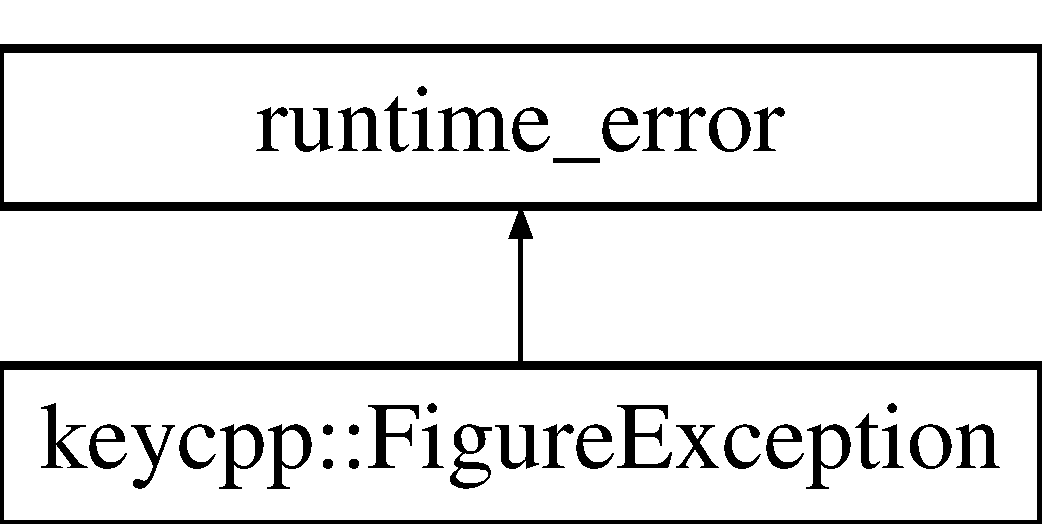
\includegraphics[height=2.000000cm]{classkeycpp_1_1_figure_exception}
\end{center}
\end{figure}
\subsection*{Public Member Functions}
\begin{DoxyCompactItemize}
\item 
\hypertarget{classkeycpp_1_1_figure_exception_aacd7cab583d3eea1ddd185a8fd7b1133}{{\bfseries Figure\-Exception} (const std\-::string \&msg)}\label{classkeycpp_1_1_figure_exception_aacd7cab583d3eea1ddd185a8fd7b1133}

\end{DoxyCompactItemize}


The documentation for this class was generated from the following file\-:\begin{DoxyCompactItemize}
\item 
Figure.\-h\end{DoxyCompactItemize}

\hypertarget{class_gnuplot}{\section{Gnuplot Class Reference}
\label{class_gnuplot}\index{Gnuplot@{Gnuplot}}
}
\subsection*{Public Member Functions}
\begin{DoxyCompactItemize}
\item 
\hypertarget{class_gnuplot_a187eb517b362cf379492fe7f1621ee50}{\hyperlink{class_gnuplot_a187eb517b362cf379492fe7f1621ee50}{Gnuplot} (const std\-::string \&style=\char`\"{}points\char`\"{})}\label{class_gnuplot_a187eb517b362cf379492fe7f1621ee50}

\begin{DoxyCompactList}\small\item\em set a style during construction \end{DoxyCompactList}\item 
\hypertarget{class_gnuplot_a8ceac5808e42665c1dee305ae7ea9070}{\hyperlink{class_gnuplot_a8ceac5808e42665c1dee305ae7ea9070}{Gnuplot} (const std\-::vector$<$ double $>$ \&x, const std\-::string \&title=\char`\"{}\char`\"{}, const std\-::string \&style=\char`\"{}points\char`\"{}, const std\-::string \&labelx=\char`\"{}x\char`\"{}, const std\-::string \&labely=\char`\"{}y\char`\"{})}\label{class_gnuplot_a8ceac5808e42665c1dee305ae7ea9070}

\begin{DoxyCompactList}\small\item\em plot a single std\-::vector at one go \end{DoxyCompactList}\item 
\hypertarget{class_gnuplot_a24327b6116c71acdc195eadf665c67cb}{\hyperlink{class_gnuplot_a24327b6116c71acdc195eadf665c67cb}{Gnuplot} (const std\-::vector$<$ double $>$ \&x, const std\-::vector$<$ double $>$ \&y, const std\-::string \&title=\char`\"{}\char`\"{}, const std\-::string \&style=\char`\"{}points\char`\"{}, const std\-::string \&labelx=\char`\"{}x\char`\"{}, const std\-::string \&labely=\char`\"{}y\char`\"{})}\label{class_gnuplot_a24327b6116c71acdc195eadf665c67cb}

\begin{DoxyCompactList}\small\item\em plot pairs std\-::vector at one go \end{DoxyCompactList}\item 
\hypertarget{class_gnuplot_a14191e89154f2716608f6907975cc012}{\hyperlink{class_gnuplot_a14191e89154f2716608f6907975cc012}{Gnuplot} (const std\-::vector$<$ double $>$ \&x, const std\-::vector$<$ double $>$ \&y, const std\-::vector$<$ double $>$ \&z, const std\-::string \&title=\char`\"{}\char`\"{}, const std\-::string \&style=\char`\"{}points\char`\"{}, const std\-::string \&labelx=\char`\"{}x\char`\"{}, const std\-::string \&labely=\char`\"{}y\char`\"{}, const std\-::string \&labelz=\char`\"{}z\char`\"{})}\label{class_gnuplot_a14191e89154f2716608f6907975cc012}

\begin{DoxyCompactList}\small\item\em plot triples std\-::vector at one go \end{DoxyCompactList}\item 
\hypertarget{class_gnuplot_a78a68f621caa87d1f34324fcd093c7bd}{\hyperlink{class_gnuplot_a78a68f621caa87d1f34324fcd093c7bd}{$\sim$\-Gnuplot} ()}\label{class_gnuplot_a78a68f621caa87d1f34324fcd093c7bd}

\begin{DoxyCompactList}\small\item\em destructor\-: needed to delete temporary files \end{DoxyCompactList}\item 
\hypertarget{class_gnuplot_a07607803ede8dd5416906df0a1924fc5}{\hyperlink{class_gnuplot}{Gnuplot} \& \hyperlink{class_gnuplot_a07607803ede8dd5416906df0a1924fc5}{cmd} (const std\-::string \&cmdstr)}\label{class_gnuplot_a07607803ede8dd5416906df0a1924fc5}

\begin{DoxyCompactList}\small\item\em send a command to gnuplot \end{DoxyCompactList}\item 
\hyperlink{class_gnuplot}{Gnuplot} \& \hyperlink{class_gnuplot_afb69631c7a498077e378a3cbb56f38c8}{operator$<$$<$} (const std\-::string \&cmdstr)
\begin{DoxyCompactList}\small\item\em Sends a command to an active gnuplot session, identical to \hyperlink{class_gnuplot_a07607803ede8dd5416906df0a1924fc5}{cmd()} send a command to gnuplot using the $<$$<$ operator. \end{DoxyCompactList}\item 
\hypertarget{class_gnuplot_a356d2faaa79f08d13fec9718b776b28d}{\hyperlink{class_gnuplot}{Gnuplot} \& \hyperlink{class_gnuplot_a356d2faaa79f08d13fec9718b776b28d}{showonscreen} ()}\label{class_gnuplot_a356d2faaa79f08d13fec9718b776b28d}

\begin{DoxyCompactList}\small\item\em sets terminal type to terminal\-\_\-std \end{DoxyCompactList}\item 
\hypertarget{class_gnuplot_a1ccaa142290490429c6cd623543a914c}{\hyperlink{class_gnuplot}{Gnuplot} \& \hyperlink{class_gnuplot_a1ccaa142290490429c6cd623543a914c}{savetofigure} (const std\-::string filename, const std\-::string terminal=\char`\"{}ps\char`\"{})}\label{class_gnuplot_a1ccaa142290490429c6cd623543a914c}

\begin{DoxyCompactList}\small\item\em Saves a gnuplot to a file named filename. Defaults to saving pdf. \end{DoxyCompactList}\item 
\hyperlink{class_gnuplot}{Gnuplot} \& \hyperlink{class_gnuplot_acfdcda292650775ebed4683e8e1515b5}{set\-\_\-style} (const std\-::string \&stylestr=\char`\"{}points\char`\"{})
\item 
\hyperlink{class_gnuplot}{Gnuplot} \& \hyperlink{class_gnuplot_aa18386919da2ec4c994f1f9c7195d384}{set\-\_\-smooth} (const std\-::string \&stylestr=\char`\"{}csplines\char`\"{})
\item 
\hyperlink{class_gnuplot}{Gnuplot} \& \hyperlink{class_gnuplot_ad9dfbccd66dece1dbe5803605c6ab08c}{unset\-\_\-smooth} ()
\begin{DoxyCompactList}\small\item\em unset smooth attention\-: smooth is not set by default \end{DoxyCompactList}\item 
\hypertarget{class_gnuplot_a95ec1636a871447dfe99463b769339c7}{\hyperlink{class_gnuplot}{Gnuplot} \& \hyperlink{class_gnuplot_a95ec1636a871447dfe99463b769339c7}{set\-\_\-pointsize} (const double pointsize=1.\-0)}\label{class_gnuplot_a95ec1636a871447dfe99463b769339c7}

\begin{DoxyCompactList}\small\item\em scales the size of the points used in plots \end{DoxyCompactList}\item 
\hypertarget{class_gnuplot_a5416c8e81f1b9945b9631fa85a8d4f47}{\hyperlink{class_gnuplot}{Gnuplot} \& \hyperlink{class_gnuplot_a5416c8e81f1b9945b9631fa85a8d4f47}{set\-\_\-grid} ()}\label{class_gnuplot_a5416c8e81f1b9945b9631fa85a8d4f47}

\begin{DoxyCompactList}\small\item\em turns grid on/off \end{DoxyCompactList}\item 
\hypertarget{class_gnuplot_a53183e1487bc6977f0d46bf75d19b4d3}{\hyperlink{class_gnuplot}{Gnuplot} \& \hyperlink{class_gnuplot_a53183e1487bc6977f0d46bf75d19b4d3}{unset\-\_\-grid} ()}\label{class_gnuplot_a53183e1487bc6977f0d46bf75d19b4d3}

\begin{DoxyCompactList}\small\item\em grid is not set by default \end{DoxyCompactList}\item 
\hyperlink{class_gnuplot}{Gnuplot} \& \hyperlink{class_gnuplot_a67efc4d4dc46b6100d14ba2f7366ef11}{set\-\_\-multiplot} ()
\item 
\hyperlink{class_gnuplot}{Gnuplot} \& \hyperlink{class_gnuplot_aad76cdec16cfb5fdf82f45ed2786f4d8}{unset\-\_\-multiplot} ()
\item 
\hypertarget{class_gnuplot_a671cbe7b18a267ea59f532c83a0035f6}{\hyperlink{class_gnuplot}{Gnuplot} \& \hyperlink{class_gnuplot_a671cbe7b18a267ea59f532c83a0035f6}{set\-\_\-samples} (const int samples=100)}\label{class_gnuplot_a671cbe7b18a267ea59f532c83a0035f6}

\begin{DoxyCompactList}\small\item\em set sampling rate of functions, or for interpolating data \end{DoxyCompactList}\item 
\hypertarget{class_gnuplot_ab810fa4c02fb49ae197786c305b78702}{\hyperlink{class_gnuplot}{Gnuplot} \& \hyperlink{class_gnuplot_ab810fa4c02fb49ae197786c305b78702}{set\-\_\-isosamples} (const int isolines=10)}\label{class_gnuplot_ab810fa4c02fb49ae197786c305b78702}

\begin{DoxyCompactList}\small\item\em set isoline density (grid) for plotting functions as surfaces (for 3d plots) \end{DoxyCompactList}\item 
\hyperlink{class_gnuplot}{Gnuplot} \& \hyperlink{class_gnuplot_a891f9800705eddc3f73886f265c009b8}{set\-\_\-hidden3d} ()
\item 
\hyperlink{class_gnuplot}{Gnuplot} \& \hyperlink{class_gnuplot_ab8688182047f746090e1e5f2a8c11c9e}{unset\-\_\-hidden3d} ()
\item 
\hyperlink{class_gnuplot}{Gnuplot} \& \hyperlink{class_gnuplot_af845efc728a90d7e10de764eff0b2423}{set\-\_\-contour} (const std\-::string \&position=\char`\"{}base\char`\"{})
\item 
\hyperlink{class_gnuplot}{Gnuplot} \& \hyperlink{class_gnuplot_a0b8522cb81e46dd4f5a22b7b48f977b1}{unset\-\_\-contour} ()
\item 
\hyperlink{class_gnuplot}{Gnuplot} \& \hyperlink{class_gnuplot_a9825bd26500e30ca88404c4807e6607a}{set\-\_\-surface} ()
\item 
\hyperlink{class_gnuplot}{Gnuplot} \& \hyperlink{class_gnuplot_a4ebddacbec61aa3e7bc4b89f508ad621}{unset\-\_\-surface} ()
\item 
\hyperlink{class_gnuplot}{Gnuplot} \& \hyperlink{class_gnuplot_ad64a717dac18167f656c4f09239973f8}{set\-\_\-legend} (const std\-::string \&position=\char`\"{}default\char`\"{})
\item 
\hyperlink{class_gnuplot}{Gnuplot} \& \hyperlink{class_gnuplot_ace901a18ab1a459213afd3ee0233b5ce}{unset\-\_\-legend} ()
\begin{DoxyCompactList}\small\item\em Switches legend off attention\-:legend is set by default. \end{DoxyCompactList}\item 
\hyperlink{class_gnuplot}{Gnuplot} \& \hyperlink{class_gnuplot_a4f93bac0e69dd83806652ca7226c6b3b}{set\-\_\-title} (const std\-::string \&title=\char`\"{}\char`\"{})
\begin{DoxyCompactList}\small\item\em sets and clears the title of a gnuplot session \end{DoxyCompactList}\item 
\hyperlink{class_gnuplot}{Gnuplot} \& \hyperlink{class_gnuplot_aca0aeb1dc0ac8d7e68ba6a15a977be28}{unset\-\_\-title} ()
\begin{DoxyCompactList}\small\item\em Clears the title of a gnuplot session The title is not set by default. \end{DoxyCompactList}\item 
\hypertarget{class_gnuplot_afcb311938827f8718f19ed52d66bad7c}{\hyperlink{class_gnuplot}{Gnuplot} \& \hyperlink{class_gnuplot_afcb311938827f8718f19ed52d66bad7c}{set\-\_\-ylabel} (const std\-::string \&label=\char`\"{}x\char`\"{})}\label{class_gnuplot_afcb311938827f8718f19ed52d66bad7c}

\begin{DoxyCompactList}\small\item\em set x axis label \end{DoxyCompactList}\item 
\hypertarget{class_gnuplot_aa93589a95aeab869ba731e2583843ae4}{\hyperlink{class_gnuplot}{Gnuplot} \& \hyperlink{class_gnuplot_aa93589a95aeab869ba731e2583843ae4}{set\-\_\-xlabel} (const std\-::string \&label=\char`\"{}y\char`\"{})}\label{class_gnuplot_aa93589a95aeab869ba731e2583843ae4}

\begin{DoxyCompactList}\small\item\em set y axis label \end{DoxyCompactList}\item 
\hypertarget{class_gnuplot_ab3206e715d20f05cc0dd1eec89ce8b07}{\hyperlink{class_gnuplot}{Gnuplot} \& \hyperlink{class_gnuplot_ab3206e715d20f05cc0dd1eec89ce8b07}{set\-\_\-zlabel} (const std\-::string \&label=\char`\"{}z\char`\"{})}\label{class_gnuplot_ab3206e715d20f05cc0dd1eec89ce8b07}

\begin{DoxyCompactList}\small\item\em set z axis label \end{DoxyCompactList}\item 
\hypertarget{class_gnuplot_a4b8d96018f2d2d4e2922d4df153d6a84}{\hyperlink{class_gnuplot}{Gnuplot} \& \hyperlink{class_gnuplot_a4b8d96018f2d2d4e2922d4df153d6a84}{set\-\_\-xrange} (const double i\-From, const double i\-To)}\label{class_gnuplot_a4b8d96018f2d2d4e2922d4df153d6a84}

\begin{DoxyCompactList}\small\item\em set axis -\/ ranges \end{DoxyCompactList}\item 
\hypertarget{class_gnuplot_a461271b7bfd4f84bdfc0055457226f28}{\hyperlink{class_gnuplot}{Gnuplot} \& \hyperlink{class_gnuplot_a461271b7bfd4f84bdfc0055457226f28}{set\-\_\-yrange} (const double i\-From, const double i\-To)}\label{class_gnuplot_a461271b7bfd4f84bdfc0055457226f28}

\begin{DoxyCompactList}\small\item\em set y-\/axis -\/ ranges \end{DoxyCompactList}\item 
\hypertarget{class_gnuplot_a7273f6a48024117b4d234d0251106e78}{\hyperlink{class_gnuplot}{Gnuplot} \& \hyperlink{class_gnuplot_a7273f6a48024117b4d234d0251106e78}{set\-\_\-zrange} (const double i\-From, const double i\-To)}\label{class_gnuplot_a7273f6a48024117b4d234d0251106e78}

\begin{DoxyCompactList}\small\item\em set z-\/axis -\/ ranges \end{DoxyCompactList}\item 
\hyperlink{class_gnuplot}{Gnuplot} \& \hyperlink{class_gnuplot_a11a62a04c203f01607c3c21a727e318d}{set\-\_\-xautoscale} ()
\item 
\hyperlink{class_gnuplot}{Gnuplot} \& \hyperlink{class_gnuplot_a5b9e1a4e68f94d418a8e9194f168b448}{set\-\_\-yautoscale} ()
\item 
\hyperlink{class_gnuplot}{Gnuplot} \& \hyperlink{class_gnuplot_aef3e84e793836158e1ddd773d1465c37}{set\-\_\-zautoscale} ()
\item 
\hypertarget{class_gnuplot_aff546fad227d93babeb5d2cc9f047b89}{\hyperlink{class_gnuplot}{Gnuplot} \& \hyperlink{class_gnuplot_aff546fad227d93babeb5d2cc9f047b89}{set\-\_\-xlogscale} (const double base=10)}\label{class_gnuplot_aff546fad227d93babeb5d2cc9f047b89}

\begin{DoxyCompactList}\small\item\em turns on/off log scaling for the specified xaxis (logscale is not set by default) \end{DoxyCompactList}\item 
\hypertarget{class_gnuplot_a201a802d2f27fece0d39809c4eb3bce0}{\hyperlink{class_gnuplot}{Gnuplot} \& \hyperlink{class_gnuplot_a201a802d2f27fece0d39809c4eb3bce0}{set\-\_\-ylogscale} (const double base=10)}\label{class_gnuplot_a201a802d2f27fece0d39809c4eb3bce0}

\begin{DoxyCompactList}\small\item\em turns on/off log scaling for the specified yaxis (logscale is not set by default) \end{DoxyCompactList}\item 
\hypertarget{class_gnuplot_a1da3838163b0dbde8809b55c5b5c56b1}{\hyperlink{class_gnuplot}{Gnuplot} \& \hyperlink{class_gnuplot_a1da3838163b0dbde8809b55c5b5c56b1}{set\-\_\-zlogscale} (const double base=10)}\label{class_gnuplot_a1da3838163b0dbde8809b55c5b5c56b1}

\begin{DoxyCompactList}\small\item\em turns on/off log scaling for the specified zaxis (logscale is not set by default) \end{DoxyCompactList}\item 
\hyperlink{class_gnuplot}{Gnuplot} \& \hyperlink{class_gnuplot_a7b178184260f1498cd0c11a197ea0ac2}{unset\-\_\-xlogscale} ()
\item 
\hyperlink{class_gnuplot}{Gnuplot} \& \hyperlink{class_gnuplot_a9217543dd49c4802b1194d42c5e10b6d}{unset\-\_\-ylogscale} ()
\item 
\hyperlink{class_gnuplot}{Gnuplot} \& \hyperlink{class_gnuplot_afa67f022ca344593b054d7f2e3406c7e}{unset\-\_\-zlogscale} ()
\item 
\hypertarget{class_gnuplot_a2228f5ab4cce2da463fc90383076a598}{\hyperlink{class_gnuplot}{Gnuplot} \& \hyperlink{class_gnuplot_a2228f5ab4cce2da463fc90383076a598}{set\-\_\-cbrange} (const double i\-From, const double i\-To)}\label{class_gnuplot_a2228f5ab4cce2da463fc90383076a598}

\begin{DoxyCompactList}\small\item\em set palette range (autoscale by default) \end{DoxyCompactList}\item 
\hyperlink{class_gnuplot}{Gnuplot} \& \hyperlink{class_gnuplot_a4fc34218cdfdd27a65b92eea1f1f9e84}{plotfile\-\_\-x} (const std\-::string \&filename, const unsigned int column=1, const std\-::string \&title=\char`\"{}\char`\"{})
\item 
{\footnotesize template$<$typename X $>$ }\\\hyperlink{class_gnuplot}{Gnuplot} \& \hyperlink{class_gnuplot_a80f3b2baae2bceff78ad005d9c3ec3fb}{plot\-\_\-x} (const X \&x, const std\-::string \&title=\char`\"{}\char`\"{})
\begin{DoxyCompactList}\small\item\em from std\-::vector \end{DoxyCompactList}\item 
\hyperlink{class_gnuplot}{Gnuplot} \& \hyperlink{class_gnuplot_a10e1fc7344bd726faa2d70cd5ced5e5e}{plotfile\-\_\-xy} (const std\-::string \&filename, const unsigned int column\-\_\-x=1, const unsigned int column\-\_\-y=2, const std\-::string \&title=\char`\"{}\char`\"{})
\item 
{\footnotesize template$<$typename X , typename Y $>$ }\\\hyperlink{class_gnuplot}{Gnuplot} \& \hyperlink{class_gnuplot_a0514a7391de6b42e79732ce746c310f7}{plot\-\_\-xy} (const X \&x, const Y \&y, const std\-::string \&title=\char`\"{}\char`\"{})
\begin{DoxyCompactList}\small\item\em from data \end{DoxyCompactList}\item 
\hyperlink{class_gnuplot}{Gnuplot} \& \hyperlink{class_gnuplot_a26cbba36864ad7f1f6683b11558e3b49}{plotfile\-\_\-xyy} (const std\-::string \&filename, const unsigned int column\-\_\-x=1, const unsigned int column\-\_\-y1=2, const unsigned int column\-\_\-y2=3, const std\-::string \&title1=\char`\"{}\char`\"{}, const std\-::string \&title2=\char`\"{}\char`\"{})
\item 
\hypertarget{class_gnuplot_ac0c275ff75d700fc8e9f55d15dea1ea3}{{\footnotesize template$<$typename X , typename Y $>$ }\\\hyperlink{class_gnuplot}{Gnuplot} \& \hyperlink{class_gnuplot_ac0c275ff75d700fc8e9f55d15dea1ea3}{plot\-\_\-xyxy} (const X \&x1, const Y \&y1, const X \&x2, const Y \&y2, const std\-::string \&title1, const std\-::string \&title2, const std\-::string \&style1=\char`\"{}\char`\"{}, const std\-::string \&style2=\char`\"{}\char`\"{})}\label{class_gnuplot_ac0c275ff75d700fc8e9f55d15dea1ea3}

\begin{DoxyCompactList}\small\item\em Plots a 2d graph from a list of doubles\-: x y. \end{DoxyCompactList}\item 
\hyperlink{class_gnuplot}{Gnuplot} \& \hyperlink{class_gnuplot_a4410bb4c65aaf43b0ad5e510da15e20f}{plotfile\-\_\-xyxy} (const std\-::string \&filename1, const std\-::string \&filename2, const unsigned int column\-\_\-x1=1, const unsigned int column\-\_\-y1=2, const unsigned int column\-\_\-x2=1, const unsigned int column\-\_\-y2=2, const std\-::string \&title1=\char`\"{}\char`\"{}, const std\-::string \&title2=\char`\"{}\char`\"{}, const std\-::string \&style1=\char`\"{}\char`\"{}, const std\-::string \&style2=\char`\"{}\char`\"{})
\item 
{\footnotesize template$<$typename X , typename Y $>$ }\\\hyperlink{class_gnuplot}{Gnuplot} \& \hyperlink{class_gnuplot_a9ac40f453f4951f5df8212612b2b5cfd}{plot\-\_\-xyy} (const X \&x, const Y \&y1, const Y \&y2, const std\-::string \&title1=\char`\"{}\char`\"{}, const std\-::string \&title2=\char`\"{}\char`\"{})
\begin{DoxyCompactList}\small\item\em from data \end{DoxyCompactList}\item 
\hyperlink{class_gnuplot}{Gnuplot} \& \hyperlink{class_gnuplot_ac2dcfa52e5758e6472c1c161f52803af}{plotfile\-\_\-xxy} (const std\-::string \&filename, const unsigned int column\-\_\-x1=1, const unsigned int column\-\_\-x2=2, const unsigned int column\-\_\-y=3, const std\-::string \&title1=\char`\"{}\char`\"{}, const std\-::string \&title2=\char`\"{}\char`\"{})
\item 
{\footnotesize template$<$typename X , typename Y $>$ }\\\hyperlink{class_gnuplot}{Gnuplot} \& \hyperlink{class_gnuplot_a5be0d83b9fe1c9123ac4868746eda15d}{plot\-\_\-xxy} (const X \&x1, const X \&x2, const Y \&y, const std\-::string \&title1=\char`\"{}\char`\"{}, const std\-::string \&title2=\char`\"{}\char`\"{})
\begin{DoxyCompactList}\small\item\em from data \end{DoxyCompactList}\item 
\hyperlink{class_gnuplot}{Gnuplot} \& \hyperlink{class_gnuplot_a6446b66df4b42691a8cd4b9c2b04f250}{plotfile\-\_\-xxxxy} (const std\-::string \&filename, const unsigned int column\-\_\-x1=1, const unsigned int column\-\_\-x2=2, const unsigned int column\-\_\-x3=3, const unsigned int column\-\_\-x4=4, const unsigned int column\-\_\-y=5, const std\-::string \&title1=\char`\"{}\char`\"{}, const std\-::string \&title2=\char`\"{}\char`\"{}, const std\-::string \&title3=\char`\"{}\char`\"{}, const std\-::string \&title4=\char`\"{}\char`\"{})
\item 
{\footnotesize template$<$typename X , typename Y $>$ }\\\hyperlink{class_gnuplot}{Gnuplot} \& \hyperlink{class_gnuplot_aa4736bcf899c4b2454117f9377a707e3}{plot\-\_\-xxxxy} (const X \&x1, const X \&x2, const X \&x3, const X \&x4, const Y \&y, const std\-::string \&title1=\char`\"{}\char`\"{}, const std\-::string \&title2=\char`\"{}\char`\"{}, const std\-::string \&title3=\char`\"{}\char`\"{}, const std\-::string \&title4=\char`\"{}\char`\"{})
\begin{DoxyCompactList}\small\item\em from data \end{DoxyCompactList}\item 
\hyperlink{class_gnuplot}{Gnuplot} \& \hyperlink{class_gnuplot_afe9d44ba12f617188111ab915010f3ab}{plotfile\-\_\-xy\-\_\-err} (const std\-::string \&filename, const unsigned int column\-\_\-x=1, const unsigned int column\-\_\-y=2, const unsigned int column\-\_\-dy=3, const std\-::string \&title=\char`\"{}\char`\"{})
\item 
{\footnotesize template$<$typename X , typename Y , typename E $>$ }\\\hyperlink{class_gnuplot}{Gnuplot} \& \hyperlink{class_gnuplot_a3c5d382eba33f92b26ba85f201bc7dea}{plot\-\_\-xy\-\_\-err} (const X \&x, const Y \&y, const E \&dy, const std\-::string \&title=\char`\"{}\char`\"{})
\begin{DoxyCompactList}\small\item\em from data \end{DoxyCompactList}\item 
\hyperlink{class_gnuplot}{Gnuplot} \& \hyperlink{class_gnuplot_a9dbde2a91eb816481657f3a22c9b0046}{plotfile\-\_\-xyz} (const std\-::string \&filename, const unsigned int column\-\_\-x=1, const unsigned int column\-\_\-y=2, const unsigned int column\-\_\-z=3, const std\-::string \&title=\char`\"{}\char`\"{})
\item 
\hypertarget{class_gnuplot_af89cb366fa7d09ffc1c351516ae54df5}{{\footnotesize template$<$typename X , typename Y , typename Z $>$ }\\\hyperlink{class_gnuplot}{Gnuplot} \& \hyperlink{class_gnuplot_af89cb366fa7d09ffc1c351516ae54df5}{plot\-\_\-xyz} (const X \&x, const Y \&y, const Z \&z, const std\-::string \&title=\char`\"{}\char`\"{})}\label{class_gnuplot_af89cb366fa7d09ffc1c351516ae54df5}

\begin{DoxyCompactList}\small\item\em from std\-::vector \end{DoxyCompactList}\item 
\hypertarget{class_gnuplot_a51ea5105eb87285820bb93910f8d346c}{\hyperlink{class_gnuplot}{Gnuplot} \& \hyperlink{class_gnuplot_a51ea5105eb87285820bb93910f8d346c}{plot\-\_\-slope} (const double a, const double b, const std\-::string \&title=\char`\"{}\char`\"{})}\label{class_gnuplot_a51ea5105eb87285820bb93910f8d346c}

\begin{DoxyCompactList}\small\item\em plot an equation of the form\-: y = ax + b, you supply a and b \end{DoxyCompactList}\item 
\hyperlink{class_gnuplot}{Gnuplot} \& \hyperlink{class_gnuplot_a42dfb8c9d4636745c7be277ed818e849}{plot\-\_\-equation} (const std\-::string \&equation, const std\-::string \&title=\char`\"{}\char`\"{})
\item 
\hyperlink{class_gnuplot}{Gnuplot} \& \hyperlink{class_gnuplot_a79aed3a6927f7d1d3497cba441e8a943}{plot\-\_\-equation3d} (const std\-::string \&equation, const std\-::string \&title=\char`\"{}\char`\"{})
\item 
\hyperlink{class_gnuplot}{Gnuplot} \& \hyperlink{class_gnuplot_aae22c0470a6fbbc1f5e84dec8d023381}{plot\-\_\-image} (const unsigned char $\ast$uc\-Pic\-Buf, const unsigned int i\-Width, const unsigned int i\-Height, const std\-::string \&title=\char`\"{}\char`\"{})
\begin{DoxyCompactList}\small\item\em plot image \end{DoxyCompactList}\item 
\hyperlink{class_gnuplot}{Gnuplot} \& \hyperlink{class_gnuplot_a34c1b3e877d246a841a29f857a29f502}{replot} (void)
\begin{DoxyCompactList}\small\item\em replot repeats the last plot or splot command. this can be useful for viewing a plot with different set options, or when generating the same plot for several devices (showonscreen, \end{DoxyCompactList}\item 
\hypertarget{class_gnuplot_a6797761712d3c311e3685bcccba65dd4}{\hyperlink{class_gnuplot}{Gnuplot} \& \hyperlink{class_gnuplot_a6797761712d3c311e3685bcccba65dd4}{reset\-\_\-plot} ()}\label{class_gnuplot_a6797761712d3c311e3685bcccba65dd4}

\begin{DoxyCompactList}\small\item\em resets a gnuplot session (next plot will erase previous ones) \end{DoxyCompactList}\item 
\hypertarget{class_gnuplot_a9aedfe8371083a1a3ac2b9493810049c}{\hyperlink{class_gnuplot}{Gnuplot} \& \hyperlink{class_gnuplot_a9aedfe8371083a1a3ac2b9493810049c}{reset\-\_\-all} ()}\label{class_gnuplot_a9aedfe8371083a1a3ac2b9493810049c}

\begin{DoxyCompactList}\small\item\em resets a gnuplot session and sets all variables to default \end{DoxyCompactList}\item 
\hypertarget{class_gnuplot_a2e449552587b0055f40f4ee079d62a8d}{void \hyperlink{class_gnuplot_a2e449552587b0055f40f4ee079d62a8d}{remove\-\_\-tmpfiles} ()}\label{class_gnuplot_a2e449552587b0055f40f4ee079d62a8d}

\begin{DoxyCompactList}\small\item\em deletes temporary files \end{DoxyCompactList}\item 
bool \hyperlink{class_gnuplot_a3135ffebb308b50c4f3178a62b23ab03}{is\-\_\-valid} ()
\begin{DoxyCompactList}\small\item\em Is the gnuplot session valid ?? \end{DoxyCompactList}\end{DoxyCompactItemize}
\subsection*{Static Public Member Functions}
\begin{DoxyCompactItemize}
\item 
static bool \hyperlink{class_gnuplot_a67cae885c26ced821e335d98986f1967}{set\-\_\-\-G\-N\-U\-Plot\-Path} (const std\-::string \&path)
\begin{DoxyCompactList}\small\item\em optional function\-: set \hyperlink{class_gnuplot}{Gnuplot} path manual attention\-: for windows\-: path with slash '/' not backslash '\textbackslash{}' \end{DoxyCompactList}\item 
static void \hyperlink{class_gnuplot_a21feba7a3916708b742c3dc25850ab2f}{set\-\_\-terminal\-\_\-std} (const std\-::string \&type)
\end{DoxyCompactItemize}


\subsection{Member Function Documentation}
\hypertarget{class_gnuplot_a3135ffebb308b50c4f3178a62b23ab03}{\index{Gnuplot@{Gnuplot}!is\-\_\-valid@{is\-\_\-valid}}
\index{is\-\_\-valid@{is\-\_\-valid}!Gnuplot@{Gnuplot}}
\subsubsection[{is\-\_\-valid}]{\setlength{\rightskip}{0pt plus 5cm}bool Gnuplot\-::is\-\_\-valid (
\begin{DoxyParamCaption}
{}
\end{DoxyParamCaption}
)\hspace{0.3cm}{\ttfamily [inline]}}}\label{class_gnuplot_a3135ffebb308b50c4f3178a62b23ab03}

\begin{DoxyParams}{Parameters}
{\em \&mdash;} & \\
\hline
\end{DoxyParams}
\begin{DoxyReturn}{Returns}
true if valid, false if not 
\end{DoxyReturn}
\hypertarget{class_gnuplot_afb69631c7a498077e378a3cbb56f38c8}{\index{Gnuplot@{Gnuplot}!operator$<$$<$@{operator$<$$<$}}
\index{operator$<$$<$@{operator$<$$<$}!Gnuplot@{Gnuplot}}
\subsubsection[{operator$<$$<$}]{\setlength{\rightskip}{0pt plus 5cm}{\bf Gnuplot}\& Gnuplot\-::operator$<$$<$ (
\begin{DoxyParamCaption}
\item[{const std\-::string \&}]{cmdstr}
\end{DoxyParamCaption}
)\hspace{0.3cm}{\ttfamily [inline]}}}\label{class_gnuplot_afb69631c7a498077e378a3cbb56f38c8}

\begin{DoxyParams}{Parameters}
{\em cmdstr} & --$>$ the command string\\
\hline
\end{DoxyParams}
\begin{DoxyReturn}{Returns}
$<$-- a reference to the gnuplot object 
\end{DoxyReturn}
\hypertarget{class_gnuplot_a42dfb8c9d4636745c7be277ed818e849}{\index{Gnuplot@{Gnuplot}!plot\-\_\-equation@{plot\-\_\-equation}}
\index{plot\-\_\-equation@{plot\-\_\-equation}!Gnuplot@{Gnuplot}}
\subsubsection[{plot\-\_\-equation}]{\setlength{\rightskip}{0pt plus 5cm}{\bf Gnuplot} \& Gnuplot\-::plot\-\_\-equation (
\begin{DoxyParamCaption}
\item[{const std\-::string \&}]{equation, }
\item[{const std\-::string \&}]{title = {\ttfamily \char`\"{}\char`\"{}}}
\end{DoxyParamCaption}
)}}\label{class_gnuplot_a42dfb8c9d4636745c7be277ed818e849}
plot an equation supplied as a std\-::string y=f(x), write only the function f(x) not y the independent variable has to be x binary operators\-: $\ast$$\ast$ exponentiation, $\ast$ multiply, / divide, + add, -\/ substract, \% modulo unary operators\-: -\/ minus, ! factorial elementary functions\-: rand(x), abs(x), sgn(x), ceil(x), floor(x), int(x), imag(x), real(x), arg(x), sqrt(x), exp(x), log(x), log10(x), sin(x), cos(x), tan(x), asin(x), acos(x), atan(x), atan2(y,x), sinh(x), cosh(x), tanh(x), asinh(x), acosh(x), atanh(x) special functions\-: erf(x), erfc(x), inverf(x), gamma(x), igamma(a,x), lgamma(x), ibeta(p,q,x), besj0(x), besj1(x), besy0(x), besy1(x), lambertw(x) statistical fuctions\-: norm(x), invnorm(x) \hypertarget{class_gnuplot_a79aed3a6927f7d1d3497cba441e8a943}{\index{Gnuplot@{Gnuplot}!plot\-\_\-equation3d@{plot\-\_\-equation3d}}
\index{plot\-\_\-equation3d@{plot\-\_\-equation3d}!Gnuplot@{Gnuplot}}
\subsubsection[{plot\-\_\-equation3d}]{\setlength{\rightskip}{0pt plus 5cm}{\bf Gnuplot} \& Gnuplot\-::plot\-\_\-equation3d (
\begin{DoxyParamCaption}
\item[{const std\-::string \&}]{equation, }
\item[{const std\-::string \&}]{title = {\ttfamily \char`\"{}\char`\"{}}}
\end{DoxyParamCaption}
)}}\label{class_gnuplot_a79aed3a6927f7d1d3497cba441e8a943}
plot an equation supplied as a std\-::string z=f(x,y), write only the function f(x,y) not z the independent variables have to be x and y \hypertarget{class_gnuplot_aae22c0470a6fbbc1f5e84dec8d023381}{\index{Gnuplot@{Gnuplot}!plot\-\_\-image@{plot\-\_\-image}}
\index{plot\-\_\-image@{plot\-\_\-image}!Gnuplot@{Gnuplot}}
\subsubsection[{plot\-\_\-image}]{\setlength{\rightskip}{0pt plus 5cm}{\bf Gnuplot} \& Gnuplot\-::plot\-\_\-image (
\begin{DoxyParamCaption}
\item[{const unsigned char $\ast$}]{uc\-Pic\-Buf, }
\item[{const unsigned int}]{i\-Width, }
\item[{const unsigned int}]{i\-Height, }
\item[{const std\-::string \&}]{title = {\ttfamily \char`\"{}\char`\"{}}}
\end{DoxyParamCaption}
)}}\label{class_gnuplot_aae22c0470a6fbbc1f5e84dec8d023381}

\begin{DoxyItemize}
\item note that this function is not valid for versions of G\-N\-U\-Plot below 4.\-2 
\end{DoxyItemize}\hypertarget{class_gnuplot_a80f3b2baae2bceff78ad005d9c3ec3fb}{\index{Gnuplot@{Gnuplot}!plot\-\_\-x@{plot\-\_\-x}}
\index{plot\-\_\-x@{plot\-\_\-x}!Gnuplot@{Gnuplot}}
\subsubsection[{plot\-\_\-x}]{\setlength{\rightskip}{0pt plus 5cm}template$<$typename X $>$ {\bf Gnuplot} \& Gnuplot\-::plot\-\_\-x (
\begin{DoxyParamCaption}
\item[{const X \&}]{x, }
\item[{const std\-::string \&}]{title = {\ttfamily \char`\"{}\char`\"{}}}
\end{DoxyParamCaption}
)}}\label{class_gnuplot_a80f3b2baae2bceff78ad005d9c3ec3fb}
Plots a 2d graph from a list of doubles\-: x. \hypertarget{class_gnuplot_aa4736bcf899c4b2454117f9377a707e3}{\index{Gnuplot@{Gnuplot}!plot\-\_\-xxxxy@{plot\-\_\-xxxxy}}
\index{plot\-\_\-xxxxy@{plot\-\_\-xxxxy}!Gnuplot@{Gnuplot}}
\subsubsection[{plot\-\_\-xxxxy}]{\setlength{\rightskip}{0pt plus 5cm}template$<$typename X , typename Y $>$ {\bf Gnuplot} \& Gnuplot\-::plot\-\_\-xxxxy (
\begin{DoxyParamCaption}
\item[{const X \&}]{x1, }
\item[{const X \&}]{x2, }
\item[{const X \&}]{x3, }
\item[{const X \&}]{x4, }
\item[{const Y \&}]{y, }
\item[{const std\-::string \&}]{title1 = {\ttfamily \char`\"{}\char`\"{}}, }
\item[{const std\-::string \&}]{title2 = {\ttfamily \char`\"{}\char`\"{}}, }
\item[{const std\-::string \&}]{title3 = {\ttfamily \char`\"{}\char`\"{}}, }
\item[{const std\-::string \&}]{title4 = {\ttfamily \char`\"{}\char`\"{}}}
\end{DoxyParamCaption}
)}}\label{class_gnuplot_aa4736bcf899c4b2454117f9377a707e3}
Plots a 2d graph from a list of doubles\-: x y. \hypertarget{class_gnuplot_a5be0d83b9fe1c9123ac4868746eda15d}{\index{Gnuplot@{Gnuplot}!plot\-\_\-xxy@{plot\-\_\-xxy}}
\index{plot\-\_\-xxy@{plot\-\_\-xxy}!Gnuplot@{Gnuplot}}
\subsubsection[{plot\-\_\-xxy}]{\setlength{\rightskip}{0pt plus 5cm}template$<$typename X , typename Y $>$ {\bf Gnuplot} \& Gnuplot\-::plot\-\_\-xxy (
\begin{DoxyParamCaption}
\item[{const X \&}]{x1, }
\item[{const X \&}]{x2, }
\item[{const Y \&}]{y, }
\item[{const std\-::string \&}]{title1 = {\ttfamily \char`\"{}\char`\"{}}, }
\item[{const std\-::string \&}]{title2 = {\ttfamily \char`\"{}\char`\"{}}}
\end{DoxyParamCaption}
)}}\label{class_gnuplot_a5be0d83b9fe1c9123ac4868746eda15d}
Plots a 2d graph from a list of doubles\-: x y. \hypertarget{class_gnuplot_a0514a7391de6b42e79732ce746c310f7}{\index{Gnuplot@{Gnuplot}!plot\-\_\-xy@{plot\-\_\-xy}}
\index{plot\-\_\-xy@{plot\-\_\-xy}!Gnuplot@{Gnuplot}}
\subsubsection[{plot\-\_\-xy}]{\setlength{\rightskip}{0pt plus 5cm}template$<$typename X , typename Y $>$ {\bf Gnuplot} \& Gnuplot\-::plot\-\_\-xy (
\begin{DoxyParamCaption}
\item[{const X \&}]{x, }
\item[{const Y \&}]{y, }
\item[{const std\-::string \&}]{title = {\ttfamily \char`\"{}\char`\"{}}}
\end{DoxyParamCaption}
)}}\label{class_gnuplot_a0514a7391de6b42e79732ce746c310f7}
Plots a 2d graph from a list of doubles\-: x y. \hypertarget{class_gnuplot_a3c5d382eba33f92b26ba85f201bc7dea}{\index{Gnuplot@{Gnuplot}!plot\-\_\-xy\-\_\-err@{plot\-\_\-xy\-\_\-err}}
\index{plot\-\_\-xy\-\_\-err@{plot\-\_\-xy\-\_\-err}!Gnuplot@{Gnuplot}}
\subsubsection[{plot\-\_\-xy\-\_\-err}]{\setlength{\rightskip}{0pt plus 5cm}template$<$typename X , typename Y , typename E $>$ {\bf Gnuplot} \& Gnuplot\-::plot\-\_\-xy\-\_\-err (
\begin{DoxyParamCaption}
\item[{const X \&}]{x, }
\item[{const Y \&}]{y, }
\item[{const E \&}]{dy, }
\item[{const std\-::string \&}]{title = {\ttfamily \char`\"{}\char`\"{}}}
\end{DoxyParamCaption}
)}}\label{class_gnuplot_a3c5d382eba33f92b26ba85f201bc7dea}




plot x,y pairs with dy errorbars \hypertarget{class_gnuplot_a9ac40f453f4951f5df8212612b2b5cfd}{\index{Gnuplot@{Gnuplot}!plot\-\_\-xyy@{plot\-\_\-xyy}}
\index{plot\-\_\-xyy@{plot\-\_\-xyy}!Gnuplot@{Gnuplot}}
\subsubsection[{plot\-\_\-xyy}]{\setlength{\rightskip}{0pt plus 5cm}template$<$typename X , typename Y $>$ {\bf Gnuplot} \& Gnuplot\-::plot\-\_\-xyy (
\begin{DoxyParamCaption}
\item[{const X \&}]{x, }
\item[{const Y \&}]{y1, }
\item[{const Y \&}]{y2, }
\item[{const std\-::string \&}]{title1 = {\ttfamily \char`\"{}\char`\"{}}, }
\item[{const std\-::string \&}]{title2 = {\ttfamily \char`\"{}\char`\"{}}}
\end{DoxyParamCaption}
)}}\label{class_gnuplot_a9ac40f453f4951f5df8212612b2b5cfd}
Plots a 2d graph from a list of doubles\-: x y. \hypertarget{class_gnuplot_a4fc34218cdfdd27a65b92eea1f1f9e84}{\index{Gnuplot@{Gnuplot}!plotfile\-\_\-x@{plotfile\-\_\-x}}
\index{plotfile\-\_\-x@{plotfile\-\_\-x}!Gnuplot@{Gnuplot}}
\subsubsection[{plotfile\-\_\-x}]{\setlength{\rightskip}{0pt plus 5cm}{\bf Gnuplot} \& Gnuplot\-::plotfile\-\_\-x (
\begin{DoxyParamCaption}
\item[{const std\-::string \&}]{filename, }
\item[{const unsigned int}]{column = {\ttfamily 1}, }
\item[{const std\-::string \&}]{title = {\ttfamily \char`\"{}\char`\"{}}}
\end{DoxyParamCaption}
)}}\label{class_gnuplot_a4fc34218cdfdd27a65b92eea1f1f9e84}
plot a single std\-::vector\-: x from file \hypertarget{class_gnuplot_a6446b66df4b42691a8cd4b9c2b04f250}{\index{Gnuplot@{Gnuplot}!plotfile\-\_\-xxxxy@{plotfile\-\_\-xxxxy}}
\index{plotfile\-\_\-xxxxy@{plotfile\-\_\-xxxxy}!Gnuplot@{Gnuplot}}
\subsubsection[{plotfile\-\_\-xxxxy}]{\setlength{\rightskip}{0pt plus 5cm}{\bf Gnuplot} \& Gnuplot\-::plotfile\-\_\-xxxxy (
\begin{DoxyParamCaption}
\item[{const std\-::string \&}]{filename, }
\item[{const unsigned int}]{column\-\_\-x1 = {\ttfamily 1}, }
\item[{const unsigned int}]{column\-\_\-x2 = {\ttfamily 2}, }
\item[{const unsigned int}]{column\-\_\-x3 = {\ttfamily 3}, }
\item[{const unsigned int}]{column\-\_\-x4 = {\ttfamily 4}, }
\item[{const unsigned int}]{column\-\_\-y = {\ttfamily 5}, }
\item[{const std\-::string \&}]{title1 = {\ttfamily \char`\"{}\char`\"{}}, }
\item[{const std\-::string \&}]{title2 = {\ttfamily \char`\"{}\char`\"{}}, }
\item[{const std\-::string \&}]{title3 = {\ttfamily \char`\"{}\char`\"{}}, }
\item[{const std\-::string \&}]{title4 = {\ttfamily \char`\"{}\char`\"{}}}
\end{DoxyParamCaption}
)}}\label{class_gnuplot_a6446b66df4b42691a8cd4b9c2b04f250}
plot x,y pairs\-: x1 x2 x3 x4 y from file \hypertarget{class_gnuplot_ac2dcfa52e5758e6472c1c161f52803af}{\index{Gnuplot@{Gnuplot}!plotfile\-\_\-xxy@{plotfile\-\_\-xxy}}
\index{plotfile\-\_\-xxy@{plotfile\-\_\-xxy}!Gnuplot@{Gnuplot}}
\subsubsection[{plotfile\-\_\-xxy}]{\setlength{\rightskip}{0pt plus 5cm}{\bf Gnuplot} \& Gnuplot\-::plotfile\-\_\-xxy (
\begin{DoxyParamCaption}
\item[{const std\-::string \&}]{filename, }
\item[{const unsigned int}]{column\-\_\-x1 = {\ttfamily 1}, }
\item[{const unsigned int}]{column\-\_\-x2 = {\ttfamily 2}, }
\item[{const unsigned int}]{column\-\_\-y = {\ttfamily 3}, }
\item[{const std\-::string \&}]{title1 = {\ttfamily \char`\"{}\char`\"{}}, }
\item[{const std\-::string \&}]{title2 = {\ttfamily \char`\"{}\char`\"{}}}
\end{DoxyParamCaption}
)}}\label{class_gnuplot_ac2dcfa52e5758e6472c1c161f52803af}
plot x,y pairs\-: x1 x2 y from file \hypertarget{class_gnuplot_a10e1fc7344bd726faa2d70cd5ced5e5e}{\index{Gnuplot@{Gnuplot}!plotfile\-\_\-xy@{plotfile\-\_\-xy}}
\index{plotfile\-\_\-xy@{plotfile\-\_\-xy}!Gnuplot@{Gnuplot}}
\subsubsection[{plotfile\-\_\-xy}]{\setlength{\rightskip}{0pt plus 5cm}{\bf Gnuplot} \& Gnuplot\-::plotfile\-\_\-xy (
\begin{DoxyParamCaption}
\item[{const std\-::string \&}]{filename, }
\item[{const unsigned int}]{column\-\_\-x = {\ttfamily 1}, }
\item[{const unsigned int}]{column\-\_\-y = {\ttfamily 2}, }
\item[{const std\-::string \&}]{title = {\ttfamily \char`\"{}\char`\"{}}}
\end{DoxyParamCaption}
)}}\label{class_gnuplot_a10e1fc7344bd726faa2d70cd5ced5e5e}
plot x,y pairs\-: x y from file \hypertarget{class_gnuplot_afe9d44ba12f617188111ab915010f3ab}{\index{Gnuplot@{Gnuplot}!plotfile\-\_\-xy\-\_\-err@{plotfile\-\_\-xy\-\_\-err}}
\index{plotfile\-\_\-xy\-\_\-err@{plotfile\-\_\-xy\-\_\-err}!Gnuplot@{Gnuplot}}
\subsubsection[{plotfile\-\_\-xy\-\_\-err}]{\setlength{\rightskip}{0pt plus 5cm}{\bf Gnuplot} \& Gnuplot\-::plotfile\-\_\-xy\-\_\-err (
\begin{DoxyParamCaption}
\item[{const std\-::string \&}]{filename, }
\item[{const unsigned int}]{column\-\_\-x = {\ttfamily 1}, }
\item[{const unsigned int}]{column\-\_\-y = {\ttfamily 2}, }
\item[{const unsigned int}]{column\-\_\-dy = {\ttfamily 3}, }
\item[{const std\-::string \&}]{title = {\ttfamily \char`\"{}\char`\"{}}}
\end{DoxyParamCaption}
)}}\label{class_gnuplot_afe9d44ba12f617188111ab915010f3ab}
plot x,y pairs with dy errorbars\-: x y dy from file \hypertarget{class_gnuplot_a4410bb4c65aaf43b0ad5e510da15e20f}{\index{Gnuplot@{Gnuplot}!plotfile\-\_\-xyxy@{plotfile\-\_\-xyxy}}
\index{plotfile\-\_\-xyxy@{plotfile\-\_\-xyxy}!Gnuplot@{Gnuplot}}
\subsubsection[{plotfile\-\_\-xyxy}]{\setlength{\rightskip}{0pt plus 5cm}{\bf Gnuplot} \& Gnuplot\-::plotfile\-\_\-xyxy (
\begin{DoxyParamCaption}
\item[{const std\-::string \&}]{filename1, }
\item[{const std\-::string \&}]{filename2, }
\item[{const unsigned int}]{column\-\_\-x1 = {\ttfamily 1}, }
\item[{const unsigned int}]{column\-\_\-y1 = {\ttfamily 2}, }
\item[{const unsigned int}]{column\-\_\-x2 = {\ttfamily 1}, }
\item[{const unsigned int}]{column\-\_\-y2 = {\ttfamily 2}, }
\item[{const std\-::string \&}]{title1 = {\ttfamily \char`\"{}\char`\"{}}, }
\item[{const std\-::string \&}]{title2 = {\ttfamily \char`\"{}\char`\"{}}, }
\item[{const std\-::string \&}]{style1 = {\ttfamily \char`\"{}\char`\"{}}, }
\item[{const std\-::string \&}]{style2 = {\ttfamily \char`\"{}\char`\"{}}}
\end{DoxyParamCaption}
)}}\label{class_gnuplot_a4410bb4c65aaf43b0ad5e510da15e20f}
plot x,y pairs\-: x y from file \hypertarget{class_gnuplot_a26cbba36864ad7f1f6683b11558e3b49}{\index{Gnuplot@{Gnuplot}!plotfile\-\_\-xyy@{plotfile\-\_\-xyy}}
\index{plotfile\-\_\-xyy@{plotfile\-\_\-xyy}!Gnuplot@{Gnuplot}}
\subsubsection[{plotfile\-\_\-xyy}]{\setlength{\rightskip}{0pt plus 5cm}{\bf Gnuplot} \& Gnuplot\-::plotfile\-\_\-xyy (
\begin{DoxyParamCaption}
\item[{const std\-::string \&}]{filename, }
\item[{const unsigned int}]{column\-\_\-x = {\ttfamily 1}, }
\item[{const unsigned int}]{column\-\_\-y1 = {\ttfamily 2}, }
\item[{const unsigned int}]{column\-\_\-y2 = {\ttfamily 3}, }
\item[{const std\-::string \&}]{title1 = {\ttfamily \char`\"{}\char`\"{}}, }
\item[{const std\-::string \&}]{title2 = {\ttfamily \char`\"{}\char`\"{}}}
\end{DoxyParamCaption}
)}}\label{class_gnuplot_a26cbba36864ad7f1f6683b11558e3b49}
plot x,y pairs\-: x y1 y2 from file \hypertarget{class_gnuplot_a9dbde2a91eb816481657f3a22c9b0046}{\index{Gnuplot@{Gnuplot}!plotfile\-\_\-xyz@{plotfile\-\_\-xyz}}
\index{plotfile\-\_\-xyz@{plotfile\-\_\-xyz}!Gnuplot@{Gnuplot}}
\subsubsection[{plotfile\-\_\-xyz}]{\setlength{\rightskip}{0pt plus 5cm}{\bf Gnuplot} \& Gnuplot\-::plotfile\-\_\-xyz (
\begin{DoxyParamCaption}
\item[{const std\-::string \&}]{filename, }
\item[{const unsigned int}]{column\-\_\-x = {\ttfamily 1}, }
\item[{const unsigned int}]{column\-\_\-y = {\ttfamily 2}, }
\item[{const unsigned int}]{column\-\_\-z = {\ttfamily 3}, }
\item[{const std\-::string \&}]{title = {\ttfamily \char`\"{}\char`\"{}}}
\end{DoxyParamCaption}
)}}\label{class_gnuplot_a9dbde2a91eb816481657f3a22c9b0046}
plot x,y,z triples\-: x y z from file \hypertarget{class_gnuplot_a34c1b3e877d246a841a29f857a29f502}{\index{Gnuplot@{Gnuplot}!replot@{replot}}
\index{replot@{replot}!Gnuplot@{Gnuplot}}
\subsubsection[{replot}]{\setlength{\rightskip}{0pt plus 5cm}{\bf Gnuplot}\& Gnuplot\-::replot (
\begin{DoxyParamCaption}
\item[{void}]{}
\end{DoxyParamCaption}
)\hspace{0.3cm}{\ttfamily [inline]}}}\label{class_gnuplot_a34c1b3e877d246a841a29f857a29f502}

\begin{DoxyParams}{Parameters}
{\em \&mdash;} & \\
\hline
\end{DoxyParams}
\begin{DoxyReturn}{Returns}
--- 
\end{DoxyReturn}
\hypertarget{class_gnuplot_af845efc728a90d7e10de764eff0b2423}{\index{Gnuplot@{Gnuplot}!set\-\_\-contour@{set\-\_\-contour}}
\index{set\-\_\-contour@{set\-\_\-contour}!Gnuplot@{Gnuplot}}
\subsubsection[{set\-\_\-contour}]{\setlength{\rightskip}{0pt plus 5cm}{\bf Gnuplot} \& Gnuplot\-::set\-\_\-contour (
\begin{DoxyParamCaption}
\item[{const std\-::string \&}]{position = {\ttfamily \char`\"{}base\char`\"{}}}
\end{DoxyParamCaption}
)}}\label{class_gnuplot_af845efc728a90d7e10de764eff0b2423}
enables/disables contour drawing for surfaces (for 3d plot) base, surface, both \hypertarget{class_gnuplot_a67cae885c26ced821e335d98986f1967}{\index{Gnuplot@{Gnuplot}!set\-\_\-\-G\-N\-U\-Plot\-Path@{set\-\_\-\-G\-N\-U\-Plot\-Path}}
\index{set\-\_\-\-G\-N\-U\-Plot\-Path@{set\-\_\-\-G\-N\-U\-Plot\-Path}!Gnuplot@{Gnuplot}}
\subsubsection[{set\-\_\-\-G\-N\-U\-Plot\-Path}]{\setlength{\rightskip}{0pt plus 5cm}bool Gnuplot\-::set\-\_\-\-G\-N\-U\-Plot\-Path (
\begin{DoxyParamCaption}
\item[{const std\-::string \&}]{path}
\end{DoxyParamCaption}
)\hspace{0.3cm}{\ttfamily [static]}}}\label{class_gnuplot_a67cae885c26ced821e335d98986f1967}

\begin{DoxyParams}{Parameters}
{\em path} & --$>$ the gnuplot path\\
\hline
\end{DoxyParams}
\begin{DoxyReturn}{Returns}
true on success, false otherwise 
\end{DoxyReturn}
\hypertarget{class_gnuplot_a891f9800705eddc3f73886f265c009b8}{\index{Gnuplot@{Gnuplot}!set\-\_\-hidden3d@{set\-\_\-hidden3d}}
\index{set\-\_\-hidden3d@{set\-\_\-hidden3d}!Gnuplot@{Gnuplot}}
\subsubsection[{set\-\_\-hidden3d}]{\setlength{\rightskip}{0pt plus 5cm}{\bf Gnuplot}\& Gnuplot\-::set\-\_\-hidden3d (
\begin{DoxyParamCaption}
{}
\end{DoxyParamCaption}
)\hspace{0.3cm}{\ttfamily [inline]}}}\label{class_gnuplot_a891f9800705eddc3f73886f265c009b8}
enables/disables hidden line removal for surface plotting (for 3d plot)


\begin{DoxyParams}{Parameters}
{\em \&mdash;} & \\
\hline
\end{DoxyParams}
\begin{DoxyReturn}{Returns}
$<$-- reference to the gnuplot object 
\end{DoxyReturn}
\hypertarget{class_gnuplot_ad64a717dac18167f656c4f09239973f8}{\index{Gnuplot@{Gnuplot}!set\-\_\-legend@{set\-\_\-legend}}
\index{set\-\_\-legend@{set\-\_\-legend}!Gnuplot@{Gnuplot}}
\subsubsection[{set\-\_\-legend}]{\setlength{\rightskip}{0pt plus 5cm}{\bf Gnuplot} \& Gnuplot\-::set\-\_\-legend (
\begin{DoxyParamCaption}
\item[{const std\-::string \&}]{position = {\ttfamily \char`\"{}default\char`\"{}}}
\end{DoxyParamCaption}
)}}\label{class_gnuplot_ad64a717dac18167f656c4f09239973f8}
switches legend on/off position\-: inside/outside, left/center/right, top/center/bottom, nobox/box \hypertarget{class_gnuplot_a67efc4d4dc46b6100d14ba2f7366ef11}{\index{Gnuplot@{Gnuplot}!set\-\_\-multiplot@{set\-\_\-multiplot}}
\index{set\-\_\-multiplot@{set\-\_\-multiplot}!Gnuplot@{Gnuplot}}
\subsubsection[{set\-\_\-multiplot}]{\setlength{\rightskip}{0pt plus 5cm}{\bf Gnuplot}\& Gnuplot\-::set\-\_\-multiplot (
\begin{DoxyParamCaption}
{}
\end{DoxyParamCaption}
)\hspace{0.3cm}{\ttfamily [inline]}}}\label{class_gnuplot_a67efc4d4dc46b6100d14ba2f7366ef11}
set the mulitplot mode


\begin{DoxyParams}{Parameters}
{\em \&mdash;} & \\
\hline
\end{DoxyParams}
\begin{DoxyReturn}{Returns}
$<$-- reference to the gnuplot object 
\end{DoxyReturn}
\hypertarget{class_gnuplot_aa18386919da2ec4c994f1f9c7195d384}{\index{Gnuplot@{Gnuplot}!set\-\_\-smooth@{set\-\_\-smooth}}
\index{set\-\_\-smooth@{set\-\_\-smooth}!Gnuplot@{Gnuplot}}
\subsubsection[{set\-\_\-smooth}]{\setlength{\rightskip}{0pt plus 5cm}{\bf Gnuplot} \& Gnuplot\-::set\-\_\-smooth (
\begin{DoxyParamCaption}
\item[{const std\-::string \&}]{stylestr = {\ttfamily \char`\"{}csplines\char`\"{}}}
\end{DoxyParamCaption}
)}}\label{class_gnuplot_aa18386919da2ec4c994f1f9c7195d384}
interpolation and approximation of data, arguments\-: csplines, bezier, acsplines (for data values $>$ 0), sbezier, unique, frequency (works only with plot\-\_\-x, plot\-\_\-xy, plotfile\-\_\-x, plotfile\-\_\-xy (if smooth is set, set\-\_\-style has no effekt on data plotting) \hypertarget{class_gnuplot_acfdcda292650775ebed4683e8e1515b5}{\index{Gnuplot@{Gnuplot}!set\-\_\-style@{set\-\_\-style}}
\index{set\-\_\-style@{set\-\_\-style}!Gnuplot@{Gnuplot}}
\subsubsection[{set\-\_\-style}]{\setlength{\rightskip}{0pt plus 5cm}{\bf Gnuplot} \& Gnuplot\-::set\-\_\-style (
\begin{DoxyParamCaption}
\item[{const std\-::string \&}]{stylestr = {\ttfamily \char`\"{}points\char`\"{}}}
\end{DoxyParamCaption}
)}}\label{class_gnuplot_acfdcda292650775ebed4683e8e1515b5}
set line style (some of these styles require additional information)\-: lines, points, linespoints, impulses, dots, steps, fsteps, histeps, boxes, histograms, filledcurves \hypertarget{class_gnuplot_a9825bd26500e30ca88404c4807e6607a}{\index{Gnuplot@{Gnuplot}!set\-\_\-surface@{set\-\_\-surface}}
\index{set\-\_\-surface@{set\-\_\-surface}!Gnuplot@{Gnuplot}}
\subsubsection[{set\-\_\-surface}]{\setlength{\rightskip}{0pt plus 5cm}{\bf Gnuplot}\& Gnuplot\-::set\-\_\-surface (
\begin{DoxyParamCaption}
{}
\end{DoxyParamCaption}
)\hspace{0.3cm}{\ttfamily [inline]}}}\label{class_gnuplot_a9825bd26500e30ca88404c4807e6607a}
enables/disables the display of surfaces (for 3d plot)


\begin{DoxyParams}{Parameters}
{\em \&mdash;} & \\
\hline
\end{DoxyParams}
\begin{DoxyReturn}{Returns}
$<$-- reference to the gnuplot object 
\end{DoxyReturn}
\hypertarget{class_gnuplot_a21feba7a3916708b742c3dc25850ab2f}{\index{Gnuplot@{Gnuplot}!set\-\_\-terminal\-\_\-std@{set\-\_\-terminal\-\_\-std}}
\index{set\-\_\-terminal\-\_\-std@{set\-\_\-terminal\-\_\-std}!Gnuplot@{Gnuplot}}
\subsubsection[{set\-\_\-terminal\-\_\-std}]{\setlength{\rightskip}{0pt plus 5cm}void Gnuplot\-::set\-\_\-terminal\-\_\-std (
\begin{DoxyParamCaption}
\item[{const std\-::string \&}]{type}
\end{DoxyParamCaption}
)\hspace{0.3cm}{\ttfamily [static]}}}\label{class_gnuplot_a21feba7a3916708b742c3dc25850ab2f}
optional\-: set standart terminal, used by showonscreen defaults\-: Windows -\/ win, Linux -\/ x11, Mac -\/ aqua 
\begin{DoxyParams}{Parameters}
{\em type} & --$>$ the terminal type\\
\hline
\end{DoxyParams}
\begin{DoxyReturn}{Returns}
--- 
\end{DoxyReturn}
\hypertarget{class_gnuplot_a4f93bac0e69dd83806652ca7226c6b3b}{\index{Gnuplot@{Gnuplot}!set\-\_\-title@{set\-\_\-title}}
\index{set\-\_\-title@{set\-\_\-title}!Gnuplot@{Gnuplot}}
\subsubsection[{set\-\_\-title}]{\setlength{\rightskip}{0pt plus 5cm}{\bf Gnuplot}\& Gnuplot\-::set\-\_\-title (
\begin{DoxyParamCaption}
\item[{const std\-::string \&}]{title = {\ttfamily \char`\"{}\char`\"{}}}
\end{DoxyParamCaption}
)\hspace{0.3cm}{\ttfamily [inline]}}}\label{class_gnuplot_a4f93bac0e69dd83806652ca7226c6b3b}

\begin{DoxyParams}{Parameters}
{\em title} & --$>$ the title of the plot \mbox{[}optional, default == \char`\"{}\char`\"{}\mbox{]}\\
\hline
\end{DoxyParams}
\begin{DoxyReturn}{Returns}
$<$-- reference to the gnuplot object 
\end{DoxyReturn}
\hypertarget{class_gnuplot_a11a62a04c203f01607c3c21a727e318d}{\index{Gnuplot@{Gnuplot}!set\-\_\-xautoscale@{set\-\_\-xautoscale}}
\index{set\-\_\-xautoscale@{set\-\_\-xautoscale}!Gnuplot@{Gnuplot}}
\subsubsection[{set\-\_\-xautoscale}]{\setlength{\rightskip}{0pt plus 5cm}{\bf Gnuplot}\& Gnuplot\-::set\-\_\-xautoscale (
\begin{DoxyParamCaption}
{}
\end{DoxyParamCaption}
)\hspace{0.3cm}{\ttfamily [inline]}}}\label{class_gnuplot_a11a62a04c203f01607c3c21a727e318d}
autoscale axis (set by default) of xaxis


\begin{DoxyParams}{Parameters}
{\em \&mdash;} & \\
\hline
\end{DoxyParams}
\begin{DoxyReturn}{Returns}
$<$-- reference to the gnuplot object 
\end{DoxyReturn}
\hypertarget{class_gnuplot_a5b9e1a4e68f94d418a8e9194f168b448}{\index{Gnuplot@{Gnuplot}!set\-\_\-yautoscale@{set\-\_\-yautoscale}}
\index{set\-\_\-yautoscale@{set\-\_\-yautoscale}!Gnuplot@{Gnuplot}}
\subsubsection[{set\-\_\-yautoscale}]{\setlength{\rightskip}{0pt plus 5cm}{\bf Gnuplot}\& Gnuplot\-::set\-\_\-yautoscale (
\begin{DoxyParamCaption}
{}
\end{DoxyParamCaption}
)\hspace{0.3cm}{\ttfamily [inline]}}}\label{class_gnuplot_a5b9e1a4e68f94d418a8e9194f168b448}
autoscale axis (set by default) of yaxis


\begin{DoxyParams}{Parameters}
{\em \&mdash;} & \\
\hline
\end{DoxyParams}
\begin{DoxyReturn}{Returns}
$<$-- reference to the gnuplot object 
\end{DoxyReturn}
\hypertarget{class_gnuplot_aef3e84e793836158e1ddd773d1465c37}{\index{Gnuplot@{Gnuplot}!set\-\_\-zautoscale@{set\-\_\-zautoscale}}
\index{set\-\_\-zautoscale@{set\-\_\-zautoscale}!Gnuplot@{Gnuplot}}
\subsubsection[{set\-\_\-zautoscale}]{\setlength{\rightskip}{0pt plus 5cm}{\bf Gnuplot}\& Gnuplot\-::set\-\_\-zautoscale (
\begin{DoxyParamCaption}
{}
\end{DoxyParamCaption}
)\hspace{0.3cm}{\ttfamily [inline]}}}\label{class_gnuplot_aef3e84e793836158e1ddd773d1465c37}
autoscale axis (set by default) of zaxis


\begin{DoxyParams}{Parameters}
{\em \&mdash;} & \\
\hline
\end{DoxyParams}
\begin{DoxyReturn}{Returns}
$<$-- reference to the gnuplot object 
\end{DoxyReturn}
\hypertarget{class_gnuplot_a0b8522cb81e46dd4f5a22b7b48f977b1}{\index{Gnuplot@{Gnuplot}!unset\-\_\-contour@{unset\-\_\-contour}}
\index{unset\-\_\-contour@{unset\-\_\-contour}!Gnuplot@{Gnuplot}}
\subsubsection[{unset\-\_\-contour}]{\setlength{\rightskip}{0pt plus 5cm}{\bf Gnuplot}\& Gnuplot\-::unset\-\_\-contour (
\begin{DoxyParamCaption}
{}
\end{DoxyParamCaption}
)\hspace{0.3cm}{\ttfamily [inline]}}}\label{class_gnuplot_a0b8522cb81e46dd4f5a22b7b48f977b1}
contour is not set by default, it disables contour drawing for surfaces


\begin{DoxyParams}{Parameters}
{\em \&mdash;} & \\
\hline
\end{DoxyParams}
\begin{DoxyReturn}{Returns}
$<$-- reference to the gnuplot object 
\end{DoxyReturn}
\hypertarget{class_gnuplot_ab8688182047f746090e1e5f2a8c11c9e}{\index{Gnuplot@{Gnuplot}!unset\-\_\-hidden3d@{unset\-\_\-hidden3d}}
\index{unset\-\_\-hidden3d@{unset\-\_\-hidden3d}!Gnuplot@{Gnuplot}}
\subsubsection[{unset\-\_\-hidden3d}]{\setlength{\rightskip}{0pt plus 5cm}{\bf Gnuplot}\& Gnuplot\-::unset\-\_\-hidden3d (
\begin{DoxyParamCaption}
{}
\end{DoxyParamCaption}
)\hspace{0.3cm}{\ttfamily [inline]}}}\label{class_gnuplot_ab8688182047f746090e1e5f2a8c11c9e}
hidden3d is not set by default


\begin{DoxyParams}{Parameters}
{\em \&mdash;} & \\
\hline
\end{DoxyParams}
\begin{DoxyReturn}{Returns}
$<$-- reference to the gnuplot object 
\end{DoxyReturn}
\hypertarget{class_gnuplot_ace901a18ab1a459213afd3ee0233b5ce}{\index{Gnuplot@{Gnuplot}!unset\-\_\-legend@{unset\-\_\-legend}}
\index{unset\-\_\-legend@{unset\-\_\-legend}!Gnuplot@{Gnuplot}}
\subsubsection[{unset\-\_\-legend}]{\setlength{\rightskip}{0pt plus 5cm}{\bf Gnuplot}\& Gnuplot\-::unset\-\_\-legend (
\begin{DoxyParamCaption}
{}
\end{DoxyParamCaption}
)\hspace{0.3cm}{\ttfamily [inline]}}}\label{class_gnuplot_ace901a18ab1a459213afd3ee0233b5ce}

\begin{DoxyParams}{Parameters}
{\em \&mdash;} & \\
\hline
\end{DoxyParams}
\begin{DoxyReturn}{Returns}
$<$-- reference to the gnuplot object 
\end{DoxyReturn}
\hypertarget{class_gnuplot_aad76cdec16cfb5fdf82f45ed2786f4d8}{\index{Gnuplot@{Gnuplot}!unset\-\_\-multiplot@{unset\-\_\-multiplot}}
\index{unset\-\_\-multiplot@{unset\-\_\-multiplot}!Gnuplot@{Gnuplot}}
\subsubsection[{unset\-\_\-multiplot}]{\setlength{\rightskip}{0pt plus 5cm}{\bf Gnuplot}\& Gnuplot\-::unset\-\_\-multiplot (
\begin{DoxyParamCaption}
{}
\end{DoxyParamCaption}
)\hspace{0.3cm}{\ttfamily [inline]}}}\label{class_gnuplot_aad76cdec16cfb5fdf82f45ed2786f4d8}
unsets the mulitplot mode


\begin{DoxyParams}{Parameters}
{\em \&mdash;} & \\
\hline
\end{DoxyParams}
\begin{DoxyReturn}{Returns}
$<$-- reference to the gnuplot object 
\end{DoxyReturn}
\hypertarget{class_gnuplot_ad9dfbccd66dece1dbe5803605c6ab08c}{\index{Gnuplot@{Gnuplot}!unset\-\_\-smooth@{unset\-\_\-smooth}}
\index{unset\-\_\-smooth@{unset\-\_\-smooth}!Gnuplot@{Gnuplot}}
\subsubsection[{unset\-\_\-smooth}]{\setlength{\rightskip}{0pt plus 5cm}{\bf Gnuplot}\& Gnuplot\-::unset\-\_\-smooth (
\begin{DoxyParamCaption}
{}
\end{DoxyParamCaption}
)\hspace{0.3cm}{\ttfamily [inline]}}}\label{class_gnuplot_ad9dfbccd66dece1dbe5803605c6ab08c}

\begin{DoxyParams}{Parameters}
{\em \&mdash;} & \\
\hline
\end{DoxyParams}
\begin{DoxyReturn}{Returns}
$<$-- a reference to a gnuplot object 
\end{DoxyReturn}
\hypertarget{class_gnuplot_a4ebddacbec61aa3e7bc4b89f508ad621}{\index{Gnuplot@{Gnuplot}!unset\-\_\-surface@{unset\-\_\-surface}}
\index{unset\-\_\-surface@{unset\-\_\-surface}!Gnuplot@{Gnuplot}}
\subsubsection[{unset\-\_\-surface}]{\setlength{\rightskip}{0pt plus 5cm}{\bf Gnuplot}\& Gnuplot\-::unset\-\_\-surface (
\begin{DoxyParamCaption}
{}
\end{DoxyParamCaption}
)\hspace{0.3cm}{\ttfamily [inline]}}}\label{class_gnuplot_a4ebddacbec61aa3e7bc4b89f508ad621}
surface is set by default, it disables the display of surfaces (for 3d plot)


\begin{DoxyParams}{Parameters}
{\em \&mdash;} & \\
\hline
\end{DoxyParams}
\begin{DoxyReturn}{Returns}
$<$-- reference to the gnuplot object 
\end{DoxyReturn}
\hypertarget{class_gnuplot_aca0aeb1dc0ac8d7e68ba6a15a977be28}{\index{Gnuplot@{Gnuplot}!unset\-\_\-title@{unset\-\_\-title}}
\index{unset\-\_\-title@{unset\-\_\-title}!Gnuplot@{Gnuplot}}
\subsubsection[{unset\-\_\-title}]{\setlength{\rightskip}{0pt plus 5cm}{\bf Gnuplot}\& Gnuplot\-::unset\-\_\-title (
\begin{DoxyParamCaption}
{}
\end{DoxyParamCaption}
)\hspace{0.3cm}{\ttfamily [inline]}}}\label{class_gnuplot_aca0aeb1dc0ac8d7e68ba6a15a977be28}

\begin{DoxyParams}{Parameters}
{\em \&mdash;} & \\
\hline
\end{DoxyParams}
\begin{DoxyReturn}{Returns}
$<$-- reference to the gnuplot object 
\end{DoxyReturn}
\hypertarget{class_gnuplot_a7b178184260f1498cd0c11a197ea0ac2}{\index{Gnuplot@{Gnuplot}!unset\-\_\-xlogscale@{unset\-\_\-xlogscale}}
\index{unset\-\_\-xlogscale@{unset\-\_\-xlogscale}!Gnuplot@{Gnuplot}}
\subsubsection[{unset\-\_\-xlogscale}]{\setlength{\rightskip}{0pt plus 5cm}{\bf Gnuplot}\& Gnuplot\-::unset\-\_\-xlogscale (
\begin{DoxyParamCaption}
{}
\end{DoxyParamCaption}
)\hspace{0.3cm}{\ttfamily [inline]}}}\label{class_gnuplot_a7b178184260f1498cd0c11a197ea0ac2}
turns off log scaling for the x axis


\begin{DoxyParams}{Parameters}
{\em \&mdash;} & \\
\hline
\end{DoxyParams}
\begin{DoxyReturn}{Returns}
$<$-- reference to the gnuplot object 
\end{DoxyReturn}
\hypertarget{class_gnuplot_a9217543dd49c4802b1194d42c5e10b6d}{\index{Gnuplot@{Gnuplot}!unset\-\_\-ylogscale@{unset\-\_\-ylogscale}}
\index{unset\-\_\-ylogscale@{unset\-\_\-ylogscale}!Gnuplot@{Gnuplot}}
\subsubsection[{unset\-\_\-ylogscale}]{\setlength{\rightskip}{0pt plus 5cm}{\bf Gnuplot}\& Gnuplot\-::unset\-\_\-ylogscale (
\begin{DoxyParamCaption}
{}
\end{DoxyParamCaption}
)\hspace{0.3cm}{\ttfamily [inline]}}}\label{class_gnuplot_a9217543dd49c4802b1194d42c5e10b6d}
turns off log scaling for the y axis


\begin{DoxyParams}{Parameters}
{\em \&mdash;} & \\
\hline
\end{DoxyParams}
\begin{DoxyReturn}{Returns}
$<$-- reference to the gnuplot object 
\end{DoxyReturn}
\hypertarget{class_gnuplot_afa67f022ca344593b054d7f2e3406c7e}{\index{Gnuplot@{Gnuplot}!unset\-\_\-zlogscale@{unset\-\_\-zlogscale}}
\index{unset\-\_\-zlogscale@{unset\-\_\-zlogscale}!Gnuplot@{Gnuplot}}
\subsubsection[{unset\-\_\-zlogscale}]{\setlength{\rightskip}{0pt plus 5cm}{\bf Gnuplot}\& Gnuplot\-::unset\-\_\-zlogscale (
\begin{DoxyParamCaption}
{}
\end{DoxyParamCaption}
)\hspace{0.3cm}{\ttfamily [inline]}}}\label{class_gnuplot_afa67f022ca344593b054d7f2e3406c7e}
turns off log scaling for the z axis


\begin{DoxyParams}{Parameters}
{\em \&mdash;} & \\
\hline
\end{DoxyParams}
\begin{DoxyReturn}{Returns}
$<$-- reference to the gnuplot object 
\end{DoxyReturn}


The documentation for this class was generated from the following files\-:\begin{DoxyCompactItemize}
\item 
gnuplot\-\_\-i.\-h\item 
gnuplot\-\_\-i.\-cpp\end{DoxyCompactItemize}

\hypertarget{class_gnuplot_exception}{\section{Gnuplot\-Exception Class Reference}
\label{class_gnuplot_exception}\index{Gnuplot\-Exception@{Gnuplot\-Exception}}
}


A C++ interface to gnuplot.  




{\ttfamily \#include $<$gnuplot\-\_\-i.\-h$>$}

Inheritance diagram for Gnuplot\-Exception\-:\begin{figure}[H]
\begin{center}
\leavevmode
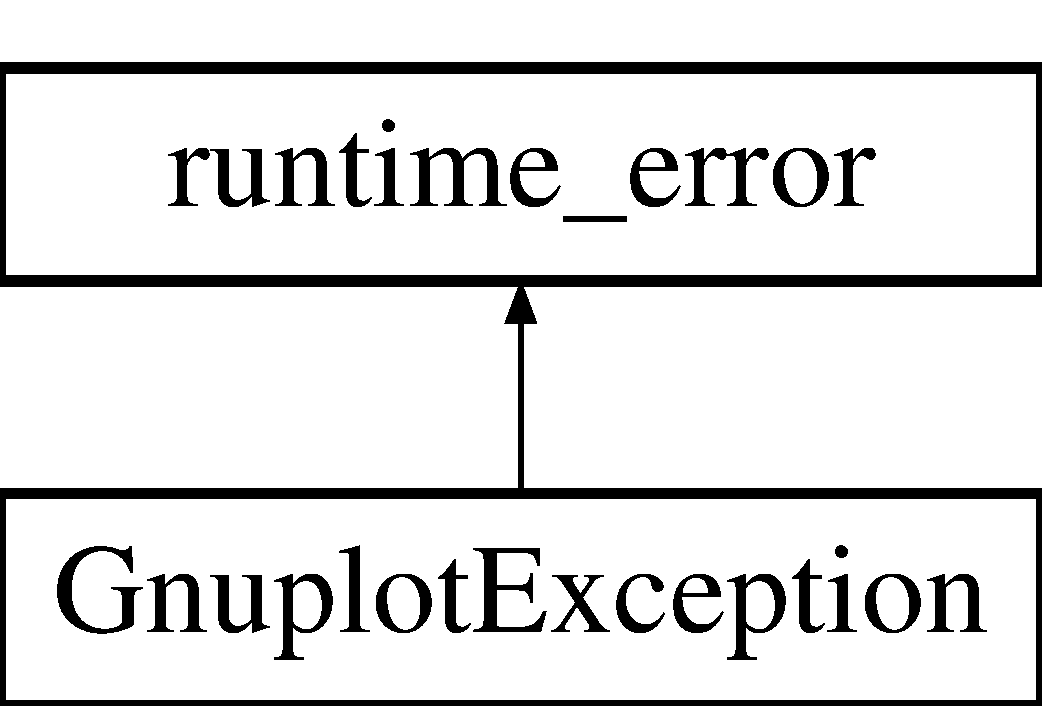
\includegraphics[height=2.000000cm]{class_gnuplot_exception}
\end{center}
\end{figure}
\subsection*{Public Member Functions}
\begin{DoxyCompactItemize}
\item 
\hypertarget{class_gnuplot_exception_a8b324a9ef4d3f75079d41ecd61c62d44}{{\bfseries Gnuplot\-Exception} (const std\-::string \&msg)}\label{class_gnuplot_exception_a8b324a9ef4d3f75079d41ecd61c62d44}

\end{DoxyCompactItemize}


\subsection{Detailed Description}
The interface uses pipes and so won't run on a system that doesn't have P\-O\-S\-I\-X pipe support Tested on Windows (Min\-G\-W and Visual C++) and Linux (G\-C\-C)

Version history\-: 0. C interface by N. Devillard (27/01/03)
\begin{DoxyEnumerate}
\item C++ interface\-: direct translation from the C interface by Rajarshi Guha (07/03/03)
\item corrections for Win32 compatibility by V. Chyzhdzenka (20/05/03)
\item some member functions added, corrections for Win32 and Linux compatibility by M. Burgis (10/03/08)
\item Some minor modifications to allow use by Key\-Cpp by J. Monschke (08/15/2013)
\end{DoxyEnumerate}

Requirements\-:
\begin{DoxyItemize}
\item gnuplot has to be installed (\href{http://www.gnuplot.info/download.html}{\tt http\-://www.\-gnuplot.\-info/download.\-html})
\item for Windows\-: set Path-\/\-Variable for \hyperlink{class_gnuplot}{Gnuplot} path (e.\-g. C\-:/program files/gnuplot/bin) or set \hyperlink{class_gnuplot}{Gnuplot} path with\-: \hyperlink{class_gnuplot_a67cae885c26ced821e335d98986f1967}{Gnuplot\-::set\-\_\-\-G\-N\-U\-Plot\-Path(const std\-::string \&path)}; 
\end{DoxyItemize}

The documentation for this class was generated from the following file\-:\begin{DoxyCompactItemize}
\item 
gnuplot\-\_\-i.\-h\end{DoxyCompactItemize}

\hypertarget{classkeycpp_1_1_key_cpp_exception}{\section{keycpp\-:\-:Key\-Cpp\-Exception Class Reference}
\label{classkeycpp_1_1_key_cpp_exception}\index{keycpp\-::\-Key\-Cpp\-Exception@{keycpp\-::\-Key\-Cpp\-Exception}}
}
Inheritance diagram for keycpp\-:\-:Key\-Cpp\-Exception\-:\begin{figure}[H]
\begin{center}
\leavevmode
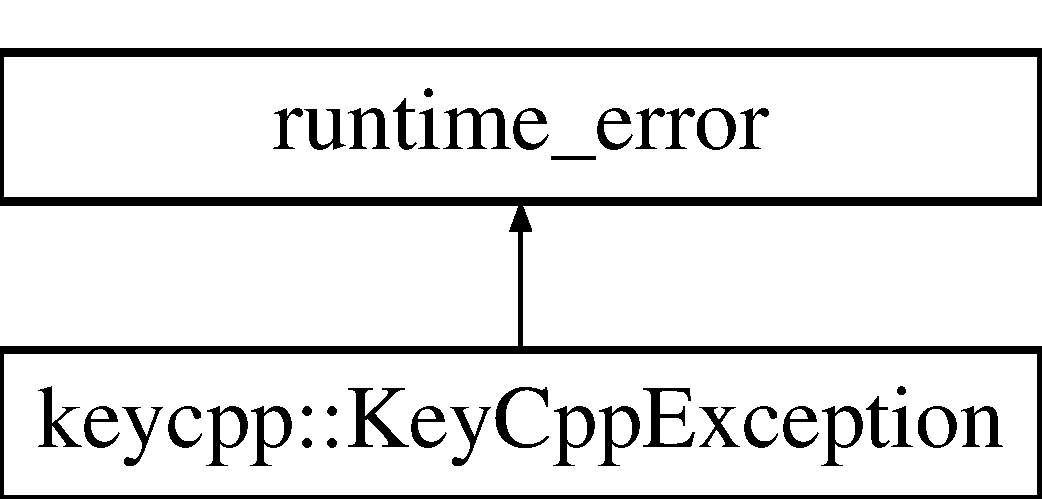
\includegraphics[height=2.000000cm]{classkeycpp_1_1_key_cpp_exception}
\end{center}
\end{figure}
\subsection*{Public Member Functions}
\begin{DoxyCompactItemize}
\item 
\hypertarget{classkeycpp_1_1_key_cpp_exception_af12dadc3f596f1e82cd65d55c2f64c65}{{\bfseries Key\-Cpp\-Exception} (const std\-::string \&msg)}\label{classkeycpp_1_1_key_cpp_exception_af12dadc3f596f1e82cd65d55c2f64c65}

\end{DoxyCompactItemize}


The documentation for this class was generated from the following file\-:\begin{DoxyCompactItemize}
\item 
\hyperlink{keycpp_8h}{keycpp.\-h}\end{DoxyCompactItemize}

\hypertarget{structkiss__fft__cpx}{\section{kiss\-\_\-fft\-\_\-cpx Struct Reference}
\label{structkiss__fft__cpx}\index{kiss\-\_\-fft\-\_\-cpx@{kiss\-\_\-fft\-\_\-cpx}}
}
\subsection*{Public Attributes}
\begin{DoxyCompactItemize}
\item 
\hypertarget{structkiss__fft__cpx_a686b6187e3e885de316908319c71ea8f}{kiss\-\_\-fft\-\_\-scalar {\bfseries r}}\label{structkiss__fft__cpx_a686b6187e3e885de316908319c71ea8f}

\item 
\hypertarget{structkiss__fft__cpx_ac1e17add2ae6b815da29d7d67b03fa70}{kiss\-\_\-fft\-\_\-scalar {\bfseries i}}\label{structkiss__fft__cpx_ac1e17add2ae6b815da29d7d67b03fa70}

\end{DoxyCompactItemize}


The documentation for this struct was generated from the following file\-:\begin{DoxyCompactItemize}
\item 
kiss\-\_\-fft.\-h\end{DoxyCompactItemize}

\hypertarget{structkiss__fft__state}{\section{kiss\-\_\-fft\-\_\-state Struct Reference}
\label{structkiss__fft__state}\index{kiss\-\_\-fft\-\_\-state@{kiss\-\_\-fft\-\_\-state}}
}
\subsection*{Public Attributes}
\begin{DoxyCompactItemize}
\item 
\hypertarget{structkiss__fft__state_aa7446bded329a40e13aef0826e349791}{int {\bfseries nfft}}\label{structkiss__fft__state_aa7446bded329a40e13aef0826e349791}

\item 
\hypertarget{structkiss__fft__state_a8faed935610ffb08bf7ad9ea8d6c81d2}{int {\bfseries inverse}}\label{structkiss__fft__state_a8faed935610ffb08bf7ad9ea8d6c81d2}

\item 
\hypertarget{structkiss__fft__state_a2d5d0897276dbac0674fae556f951d18}{int {\bfseries factors} \mbox{[}2 $\ast$M\-A\-X\-F\-A\-C\-T\-O\-R\-S\mbox{]}}\label{structkiss__fft__state_a2d5d0897276dbac0674fae556f951d18}

\item 
\hypertarget{structkiss__fft__state_aa7d1cab86ec03a8ecddfe0d91ef0bd20}{\hyperlink{structkiss__fft__cpx}{kiss\-\_\-fft\-\_\-cpx} {\bfseries twiddles} \mbox{[}1\mbox{]}}\label{structkiss__fft__state_aa7d1cab86ec03a8ecddfe0d91ef0bd20}

\end{DoxyCompactItemize}


The documentation for this struct was generated from the following file\-:\begin{DoxyCompactItemize}
\item 
\-\_\-kiss\-\_\-fft\-\_\-guts.\-h\end{DoxyCompactItemize}

\hypertarget{classkeycpp_1_1matrix}{\section{keycpp\-:\-:matrix$<$ T $>$ Class Template Reference}
\label{classkeycpp_1_1matrix}\index{keycpp\-::matrix$<$ T $>$@{keycpp\-::matrix$<$ T $>$}}
}
\subsection*{Public Member Functions}
\begin{DoxyCompactItemize}
\item 
\hypertarget{classkeycpp_1_1matrix_a7846ea93147dca75e5a8fbea7219c35d}{{\bfseries matrix} (const int \&rows, const int \&cols)}\label{classkeycpp_1_1matrix_a7846ea93147dca75e5a8fbea7219c35d}

\item 
\hypertarget{classkeycpp_1_1matrix_ad843813ecfec7c08b9259957406e94e2}{{\bfseries matrix} (const std\-::vector$<$ std\-::vector$<$ T $>$$>$ \&mat)}\label{classkeycpp_1_1matrix_ad843813ecfec7c08b9259957406e94e2}

\item 
\hypertarget{classkeycpp_1_1matrix_ad8797411bc30cc0d42e0e9b8bcc899d7}{{\bfseries matrix} (const std\-::initializer\-\_\-list$<$ std\-::initializer\-\_\-list$<$ T $>$$>$ \&lst)}\label{classkeycpp_1_1matrix_ad8797411bc30cc0d42e0e9b8bcc899d7}

\item 
\hypertarget{classkeycpp_1_1matrix_a9613f3ed2de6b240b982df895f958c56}{T \& {\bfseries operator()} (const int \&i, const int \&j)}\label{classkeycpp_1_1matrix_a9613f3ed2de6b240b982df895f958c56}

\item 
\hypertarget{classkeycpp_1_1matrix_a2c51fa98ec9a48f18af144677c36ee98}{T {\bfseries operator()} (const int \&i, const int \&j) const }\label{classkeycpp_1_1matrix_a2c51fa98ec9a48f18af144677c36ee98}

\item 
\hypertarget{classkeycpp_1_1matrix_a8a60e529610d6ad6ae5f34b8cd5199bd}{std\-::vector$<$ T $>$ {\bfseries operator$\ast$} (const std\-::vector$<$ T $>$ \&x) const }\label{classkeycpp_1_1matrix_a8a60e529610d6ad6ae5f34b8cd5199bd}

\item 
\hypertarget{classkeycpp_1_1matrix_add1f4ca03e1cce57574c905ab7ca89fe}{\hyperlink{classkeycpp_1_1matrix}{matrix}$<$ T $>$ {\bfseries operator$\ast$} (const \hyperlink{classkeycpp_1_1matrix}{matrix}$<$ T $>$ \&B) const }\label{classkeycpp_1_1matrix_add1f4ca03e1cce57574c905ab7ca89fe}

\item 
\hypertarget{classkeycpp_1_1matrix_a8c0520cf5064379afa5128cf7f660832}{\hyperlink{classkeycpp_1_1matrix}{matrix}$<$ T $>$ {\bfseries operator+} (const \hyperlink{classkeycpp_1_1matrix}{matrix}$<$ T $>$ \&B) const }\label{classkeycpp_1_1matrix_a8c0520cf5064379afa5128cf7f660832}

\item 
\hypertarget{classkeycpp_1_1matrix_a78655e73267b48e16909a68291f4c074}{\hyperlink{classkeycpp_1_1matrix}{matrix}$<$ T $>$ \& {\bfseries operator+=} (const \hyperlink{classkeycpp_1_1matrix}{matrix}$<$ T $>$ \&B)}\label{classkeycpp_1_1matrix_a78655e73267b48e16909a68291f4c074}

\item 
\hypertarget{classkeycpp_1_1matrix_a1c6cb00f8859e6486a7054f11b1c7e6a}{\hyperlink{classkeycpp_1_1matrix}{matrix}$<$ T $>$ {\bfseries operator-\/} (const \hyperlink{classkeycpp_1_1matrix}{matrix}$<$ T $>$ \&B) const }\label{classkeycpp_1_1matrix_a1c6cb00f8859e6486a7054f11b1c7e6a}

\item 
\hypertarget{classkeycpp_1_1matrix_a32a13ebb69fb5f06dd8923d942d865b4}{int {\bfseries size} (const int \&n) const }\label{classkeycpp_1_1matrix_a32a13ebb69fb5f06dd8923d942d865b4}

\item 
\hypertarget{classkeycpp_1_1matrix_ad522f701e86eafc344d8904d4f0a8f19}{bool {\bfseries empty} () const }\label{classkeycpp_1_1matrix_ad522f701e86eafc344d8904d4f0a8f19}

\item 
\hypertarget{classkeycpp_1_1matrix_a4b28c8f7b6e3d32aab1416faa9316e11}{int {\bfseries set\-Row} (const std\-::vector$<$ T $>$ \&row, const int \&i)}\label{classkeycpp_1_1matrix_a4b28c8f7b6e3d32aab1416faa9316e11}

\item 
\hypertarget{classkeycpp_1_1matrix_ac7675f496771e688a1c059b58ac975cb}{int {\bfseries set\-Last\-Row} (const std\-::vector$<$ T $>$ \&row)}\label{classkeycpp_1_1matrix_ac7675f496771e688a1c059b58ac975cb}

\item 
\hypertarget{classkeycpp_1_1matrix_aa6903fc828a5b42f7c1d9485832601aa}{int {\bfseries add\-Last\-Row} (const std\-::vector$<$ T $>$ \&row)}\label{classkeycpp_1_1matrix_aa6903fc828a5b42f7c1d9485832601aa}

\item 
\hypertarget{classkeycpp_1_1matrix_adf4d81176c098ead33c56d84421b14f5}{int {\bfseries set\-Col} (const std\-::vector$<$ T $>$ \&col, const int \&j)}\label{classkeycpp_1_1matrix_adf4d81176c098ead33c56d84421b14f5}

\item 
\hypertarget{classkeycpp_1_1matrix_a14cad5ff7a9b3079754fc83b677208ed}{std\-::vector$<$ T $>$ {\bfseries get\-Row} (const int \&i) const }\label{classkeycpp_1_1matrix_a14cad5ff7a9b3079754fc83b677208ed}

\item 
\hypertarget{classkeycpp_1_1matrix_a20002e97217bcc6382e60694bf898e1f}{std\-::vector$<$ T $>$ {\bfseries get\-Last\-Row} () const }\label{classkeycpp_1_1matrix_a20002e97217bcc6382e60694bf898e1f}

\item 
\hypertarget{classkeycpp_1_1matrix_a9c16ead5c2a61eb35c33328caa235b2f}{std\-::vector$<$ T $>$ {\bfseries get\-Col} (const int \&j) const }\label{classkeycpp_1_1matrix_a9c16ead5c2a61eb35c33328caa235b2f}

\item 
\hypertarget{classkeycpp_1_1matrix_a719eb1cb62d0cd9168abe2235235f278}{int {\bfseries reserve} (const int \&N)}\label{classkeycpp_1_1matrix_a719eb1cb62d0cd9168abe2235235f278}

\item 
\hypertarget{classkeycpp_1_1matrix_a53aaf4f54bdbebf5664b67a440f73040}{{\footnotesize template$<$$>$ }\\std\-::vector$<$ double $>$ {\bfseries operator$\ast$} (const std\-::vector$<$ double $>$ \&x) const}\label{classkeycpp_1_1matrix_a53aaf4f54bdbebf5664b67a440f73040}

\item 
\hypertarget{classkeycpp_1_1matrix_a8a9131597beafc39a3d94b59af930756}{{\footnotesize template$<$$>$ }\\std\-::vector$<$ std\-::complex\\*
$<$ double $>$ $>$ {\bfseries operator$\ast$} (const std\-::vector$<$ std\-::complex$<$ double $>$$>$ \&x) const}\label{classkeycpp_1_1matrix_a8a9131597beafc39a3d94b59af930756}

\item 
\hypertarget{classkeycpp_1_1matrix_a0e9fdbebdf1d95dd225a2bd1310cba30}{{\footnotesize template$<$$>$ }\\\hyperlink{classkeycpp_1_1matrix}{matrix}$<$ double $>$ {\bfseries operator$\ast$} (const \hyperlink{classkeycpp_1_1matrix}{matrix}$<$ double $>$ \&B) const}\label{classkeycpp_1_1matrix_a0e9fdbebdf1d95dd225a2bd1310cba30}

\item 
\hypertarget{classkeycpp_1_1matrix_a0cbaef09170a16f74ed5acefa0f8ad3a}{{\footnotesize template$<$$>$ }\\\hyperlink{classkeycpp_1_1matrix}{matrix}$<$ std\-::complex$<$ double $>$ $>$ {\bfseries operator$\ast$} (const \hyperlink{classkeycpp_1_1matrix}{matrix}$<$ std\-::complex$<$ double $>$$>$ \&B) const}\label{classkeycpp_1_1matrix_a0cbaef09170a16f74ed5acefa0f8ad3a}

\end{DoxyCompactItemize}
\subsection*{Public Attributes}
\begin{DoxyCompactItemize}
\item 
\hypertarget{classkeycpp_1_1matrix_ae2144abe57757c5a29e73aaf4d3520aa}{std\-::vector$<$ T $>$ {\bfseries m\-Data}}\label{classkeycpp_1_1matrix_ae2144abe57757c5a29e73aaf4d3520aa}

\end{DoxyCompactItemize}


The documentation for this class was generated from the following file\-:\begin{DoxyCompactItemize}
\item 
Matrix.\-h\end{DoxyCompactItemize}

\hypertarget{classkeycpp_1_1_matrix_exception}{\section{keycpp\-:\-:Matrix\-Exception Class Reference}
\label{classkeycpp_1_1_matrix_exception}\index{keycpp\-::\-Matrix\-Exception@{keycpp\-::\-Matrix\-Exception}}
}
Inheritance diagram for keycpp\-:\-:Matrix\-Exception\-:\begin{figure}[H]
\begin{center}
\leavevmode
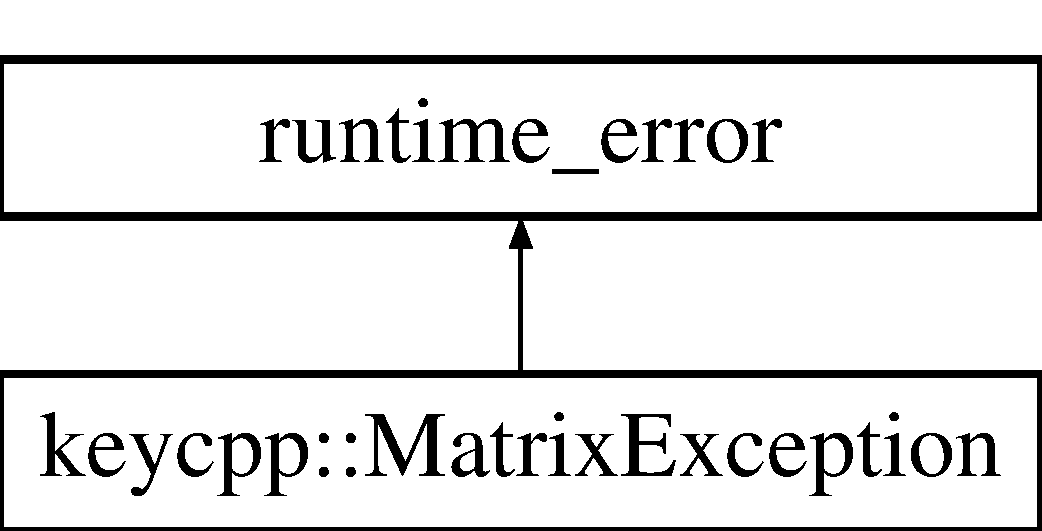
\includegraphics[height=2.000000cm]{classkeycpp_1_1_matrix_exception}
\end{center}
\end{figure}
\subsection*{Public Member Functions}
\begin{DoxyCompactItemize}
\item 
\hypertarget{classkeycpp_1_1_matrix_exception_ae558e1658f52404739cbb6fe784f196d}{{\bfseries Matrix\-Exception} (const std\-::string \&msg)}\label{classkeycpp_1_1_matrix_exception_ae558e1658f52404739cbb6fe784f196d}

\end{DoxyCompactItemize}


The documentation for this class was generated from the following file\-:\begin{DoxyCompactItemize}
\item 
Matrix.\-h\end{DoxyCompactItemize}

\hypertarget{structkeycpp_1_1observe}{\section{keycpp\-:\-:observe$<$ T, U $>$ Struct Template Reference}
\label{structkeycpp_1_1observe}\index{keycpp\-::observe$<$ T, U $>$@{keycpp\-::observe$<$ T, U $>$}}
}
\subsection*{Public Member Functions}
\begin{DoxyCompactItemize}
\item 
\hypertarget{structkeycpp_1_1observe_a88747e0078d06440401d309aba55954e}{{\bfseries observe} (std\-::vector$<$ T $>$ \&p\-\_\-y, std\-::vector$<$ U $>$ \&p\-\_\-x\-\_\-ode)}\label{structkeycpp_1_1observe_a88747e0078d06440401d309aba55954e}

\item 
\hypertarget{structkeycpp_1_1observe_a0063ab6fcada5756c6dca31ac7c17af9}{void {\bfseries operator()} (const T \&y\-\_\-temp, U x\-\_\-temp)}\label{structkeycpp_1_1observe_a0063ab6fcada5756c6dca31ac7c17af9}

\end{DoxyCompactItemize}
\subsection*{Public Attributes}
\begin{DoxyCompactItemize}
\item 
\hypertarget{structkeycpp_1_1observe_ab864306595f62009949934d352b43abf}{std\-::vector$<$ T $>$ \& {\bfseries y}}\label{structkeycpp_1_1observe_ab864306595f62009949934d352b43abf}

\item 
\hypertarget{structkeycpp_1_1observe_aecc1e14f64f33f35c50aee35cc86dac5}{std\-::vector$<$ U $>$ \& {\bfseries x\-\_\-ode}}\label{structkeycpp_1_1observe_aecc1e14f64f33f35c50aee35cc86dac5}

\end{DoxyCompactItemize}


The documentation for this struct was generated from the following file\-:\begin{DoxyCompactItemize}
\item 
keycpp.\-h\end{DoxyCompactItemize}

\hypertarget{classkeycpp_1_1_spline}{\section{keycpp\-:\-:Spline$<$ U, T $>$ Class Template Reference}
\label{classkeycpp_1_1_spline}\index{keycpp\-::\-Spline$<$ U, T $>$@{keycpp\-::\-Spline$<$ U, T $>$}}
}
\subsection*{Public Member Functions}
\begin{DoxyCompactItemize}
\item 
\hypertarget{classkeycpp_1_1_spline_a4a5f709dc92fefe7e0799c73c80234e0}{{\bfseries Spline} (int N, \hyperlink{classkeycpp_1_1vector__k}{vector\-\_\-k}$<$ U $>$ X, \hyperlink{classkeycpp_1_1vector__k}{vector\-\_\-k}$<$ T $>$ Y, \hyperlink{classkeycpp_1_1_extrap}{Extrap} extrap\-\_\-in)}\label{classkeycpp_1_1_spline_a4a5f709dc92fefe7e0799c73c80234e0}

\item 
\hypertarget{classkeycpp_1_1_spline_a8d7aaf51fd3a1c48ed43d70b2b9c10fe}{virtual \hyperlink{classkeycpp_1_1_spline_a8d7aaf51fd3a1c48ed43d70b2b9c10fe}{$\sim$\-Spline} ()}\label{classkeycpp_1_1_spline_a8d7aaf51fd3a1c48ed43d70b2b9c10fe}

\begin{DoxyCompactList}\small\item\em \hyperlink{classkeycpp_1_1_spline}{Spline} destructor, nothing needs to be done. \end{DoxyCompactList}\item 
\hypertarget{classkeycpp_1_1_spline_afcd84822df41426f4ea9da070d97b376}{int {\bfseries compute\-\_\-spline} ()}\label{classkeycpp_1_1_spline_afcd84822df41426f4ea9da070d97b376}

\item 
\hypertarget{classkeycpp_1_1_spline_a7fa452b0c1952f0a3e4160f59195d513}{T {\bfseries J} (U)}\label{classkeycpp_1_1_spline_a7fa452b0c1952f0a3e4160f59195d513}

\end{DoxyCompactItemize}


The documentation for this class was generated from the following file\-:\begin{DoxyCompactItemize}
\item 
Spline.\-h\end{DoxyCompactItemize}

\hypertarget{classkeycpp_1_1_spline_exception}{\section{keycpp\-:\-:Spline\-Exception Class Reference}
\label{classkeycpp_1_1_spline_exception}\index{keycpp\-::\-Spline\-Exception@{keycpp\-::\-Spline\-Exception}}
}
Inheritance diagram for keycpp\-:\-:Spline\-Exception\-:\begin{figure}[H]
\begin{center}
\leavevmode
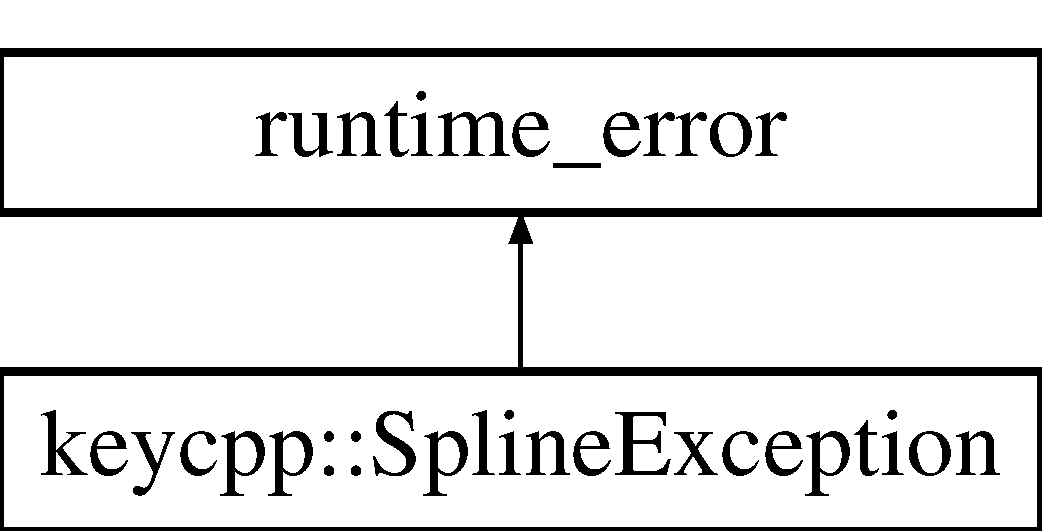
\includegraphics[height=2.000000cm]{classkeycpp_1_1_spline_exception}
\end{center}
\end{figure}
\subsection*{Public Member Functions}
\begin{DoxyCompactItemize}
\item 
\hypertarget{classkeycpp_1_1_spline_exception_a7c13b157534ec469e0b735c071192df8}{{\bfseries Spline\-Exception} (const std\-::string \&msg)}\label{classkeycpp_1_1_spline_exception_a7c13b157534ec469e0b735c071192df8}

\end{DoxyCompactItemize}


The documentation for this class was generated from the following file\-:\begin{DoxyCompactItemize}
\item 
Spline.\-h\end{DoxyCompactItemize}

\addcontentsline{toc}{part}{Index}
\printindex
\end{document}
